% ---------------------------------------------------------------
% Dataset and Exploratory Analysis
% Included from main.tex with % ---------------------------------------------------------------
% Dataset and Exploratory Analysis
% Included from main.tex with % ---------------------------------------------------------------
% Dataset and Exploratory Analysis
% Included from main.tex with % ---------------------------------------------------------------
% Dataset and Exploratory Analysis
% Included from main.tex with \input{sections/dataset_eda}
% Figures are read from ../results/figures/ (see \graphicspath in main.tex)
% ---------------------------------------------------------------

\subsection{Dataset}

We use the UJIIndoorLoc dataset~\cite{torres2014ujiindoorloc, uci_ujiindoorloc}, a public benchmark for
Wi-Fi fingerprinting collected in three buildings of Universitat Jaume I, Spain. Each row is one Wi-Fi
scan taken by a smartphone. It contains the received signal strength (RSSI) of 520 wireless access
points (WAPs), the true location of the phone, and information about who took the scan, with which
phone, and when.

RSSI values are given in dBm and range from $-104$ (very weak) to $0$ (very strong). An access point
that was not detected is recorded as $+100$. This value is a placeholder, not a measurement, and it
must be handled explicitly because otherwise it would look like the strongest possible signal.

The prediction targets are the building (3 classes) and floor (5 classes), treated as classification,
and the longitude and latitude, treated as regression. The coordinates are projected positions in
metres, so positioning error can be reported in metres. The remaining columns (\texttt{SPACEID},
\texttt{RELATIVEPOSITION}, \texttt{USERID}, \texttt{PHONEID}, \texttt{TIMESTAMP}) are not used as model
inputs; we use them only for quality checks and to design fair validation splits.

The dataset is provided as two files: a training file and a validation file. The labels of the original
competition test set were never released, so, following common practice, we use the validation file
as our held-out test set and do not use it for any modelling decision. Table~\ref{tab:summary}
summarises both files.

\begin{table}[!t]
\centering
\caption{Summary of the two data files}
\label{tab:summary}
\begin{tabular}{lrr}
\toprule
 & \textbf{Train} & \textbf{Validation} \\
\midrule
Scans (rows) & 19{,}937 & 1{,}111 \\
Buildings / floors & 3 / 5 & 3 / 5 \\
Building--floor combinations & 13 & 13 \\
Users / phones & 18 / 16 & -- / 11 \\
Collection period & May--Jun 2013 & Sep--Oct 2013 \\
Signal values $=100$ (not detected) & 96.5\% & 96.8\% \\
Median APs detected per scan & 17 & 15 \\
Scans with no AP detected & 76 & 0 \\
Exact duplicate rows & 637 & 0 \\
Scans after removing duplicates & 19{,}300 & 1{,}111 \\
\bottomrule
\end{tabular}
\end{table}

\begin{figure}[!t]
\centering
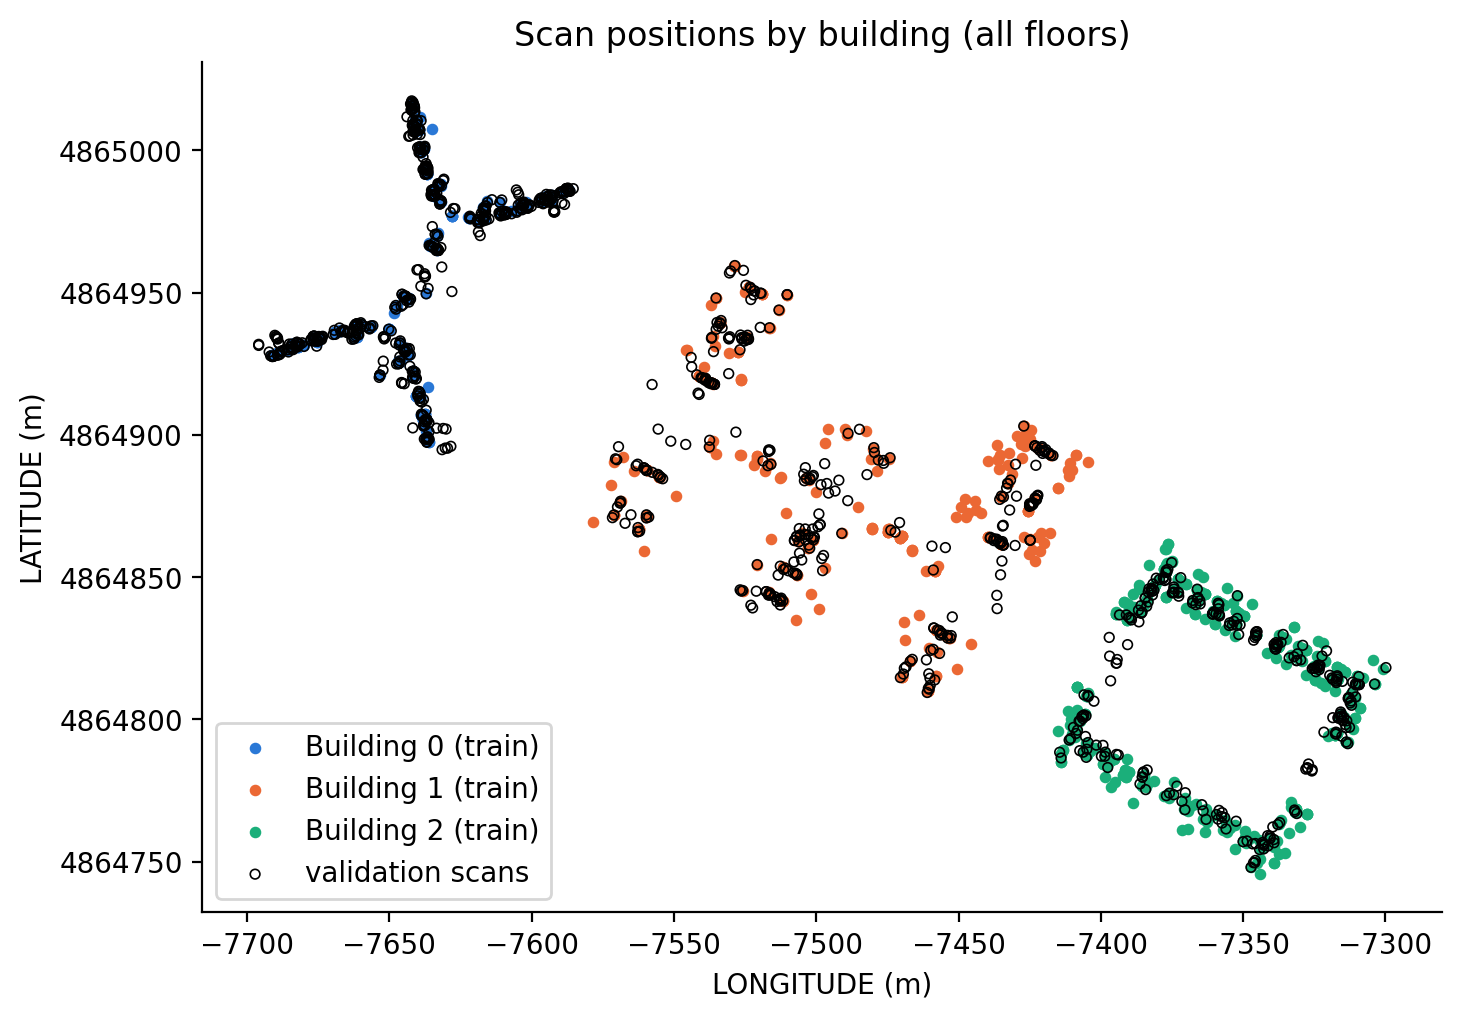
\includegraphics[width=\columnwidth]{eda_map_by_building.png}
\caption{Scan positions in the training file, coloured by building, with validation scans shown as
black circles. The three buildings occupy separate areas of the campus.}
\label{fig:map}
\end{figure}

\subsection{Data Quality}

Table~\ref{tab:quality} lists the quality checks and their outcome. The data is reliable overall: all
real RSSI values lie in the documented range, the labels are valid (floor~4 exists only in
building~2, the only five-floor building), and the three buildings are spatially separate
(Fig.~\ref{fig:map}).

A few issues require preprocessing decisions. First, the training file contains 637 exact duplicate
rows (3.2\%), 622 of them from a single user. None has conflicting labels, but copies falling on both
sides of a split would inflate validation scores, so we remove them. All results below use the remaining
19{,}300 training scans. Second, 73 of these scans detected no access point at all and therefore carry
no information; 59 of them come from a single user and phone, which points to a faulty recording
session. Third, 55 access points are never detected in the training file, so their columns are
constant and can be removed. The same 55 access points do appear in the validation file, while 153
access points seen in training never appear in validation, which shows that the Wi-Fi infrastructure
changed between the two collections.

Finally, 775 readings stronger than $-30$~dBm occur in 492 training scans, whereas the strongest
validation reading is $-34$~dBm. 87\% of these scans come from one device (phone~19), so we treat them
as a device artefact; capping readings at $-30$~dBm removes them.

\begin{table}[!t]
\centering
\caption{Data-quality checks on the training file}
\label{tab:quality}
\setlength{\tabcolsep}{3pt}
\begin{tabular}{p{0.27\columnwidth}p{0.40\columnwidth}p{0.27\columnwidth}}
\toprule
\textbf{Check} & \textbf{Result} & \textbf{Action} \\
\midrule
RSSI range & All real values in $[-104, 0]$ & None \\
Labels & Valid; floor 4 only in building 2 & None \\
Empty scans & 73 (59 from one device) & Remove \\
Duplicates & 637 exact duplicates (622 from one user) & Removed \\
Never-detected APs & 55 constant columns & Drop \\
Very strong readings & 492 scans, 87\% from phone 19 & Cap at $-30$ dBm \\
Validation metadata & User, room and position columns are always 0 & Never use as inputs \\
\bottomrule
\end{tabular}
\end{table}

\subsection{Label Distributions}

Fig.~\ref{fig:buildings} shows that the two files emphasise different buildings: building~2 makes up
47.2\% of the training scans, while building~0 makes up 48.2\% of the validation scans. Overall
validation accuracy is therefore driven mostly by building~0, and we report results per building as
well as overall.

Class imbalance is moderate (Fig.~\ref{fig:classes}). Every building--floor combination has at least
727 training scans, recorded at 50--113 distinct positions with about 20 scans per position. The
largest combination (building~2, floor~3) has 3.7 times as many scans as the smallest (building~2,
floor~4). A classifier that always predicts the most frequent class would reach 47.2\% building
accuracy and 26.1\% floor accuracy; these are the baselines any model must clearly exceed. Because of
the imbalance, we report macro-F1 alongside accuracy.

\begin{figure}[!t]
\centering
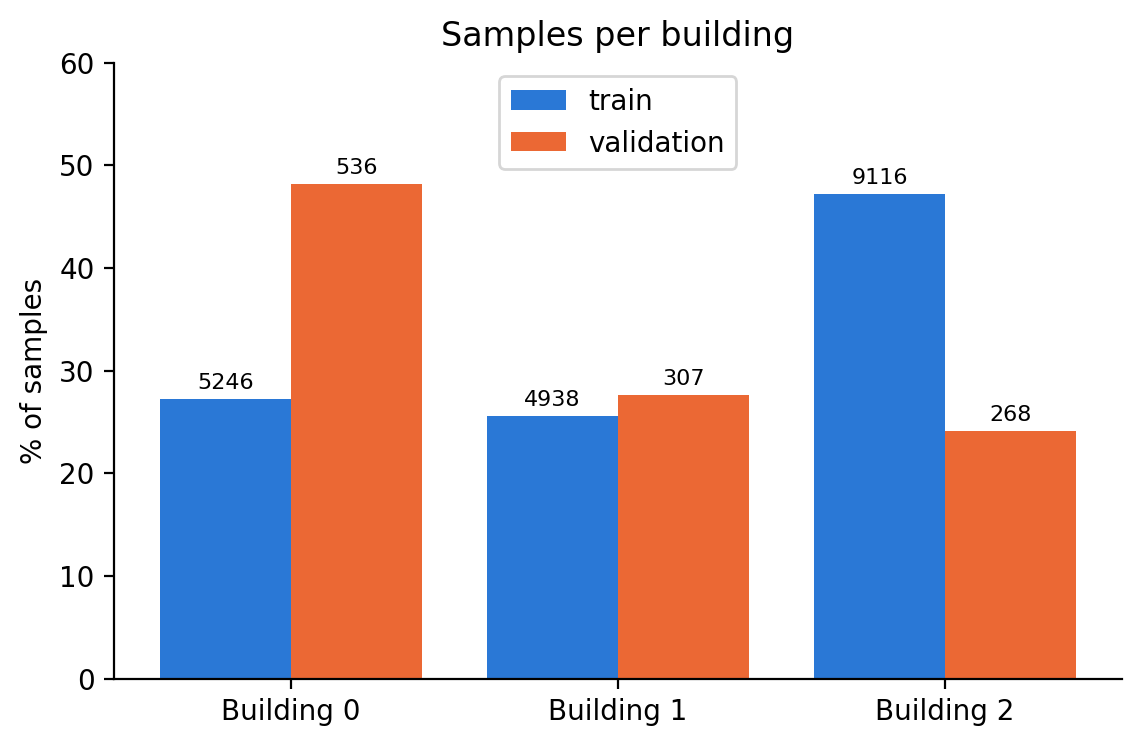
\includegraphics[width=0.9\columnwidth]{eda_samples_per_building.png}
\caption{Share of scans per building in each file (counts above the bars).}
\label{fig:buildings}
\end{figure}

\begin{figure}[!t]
\centering
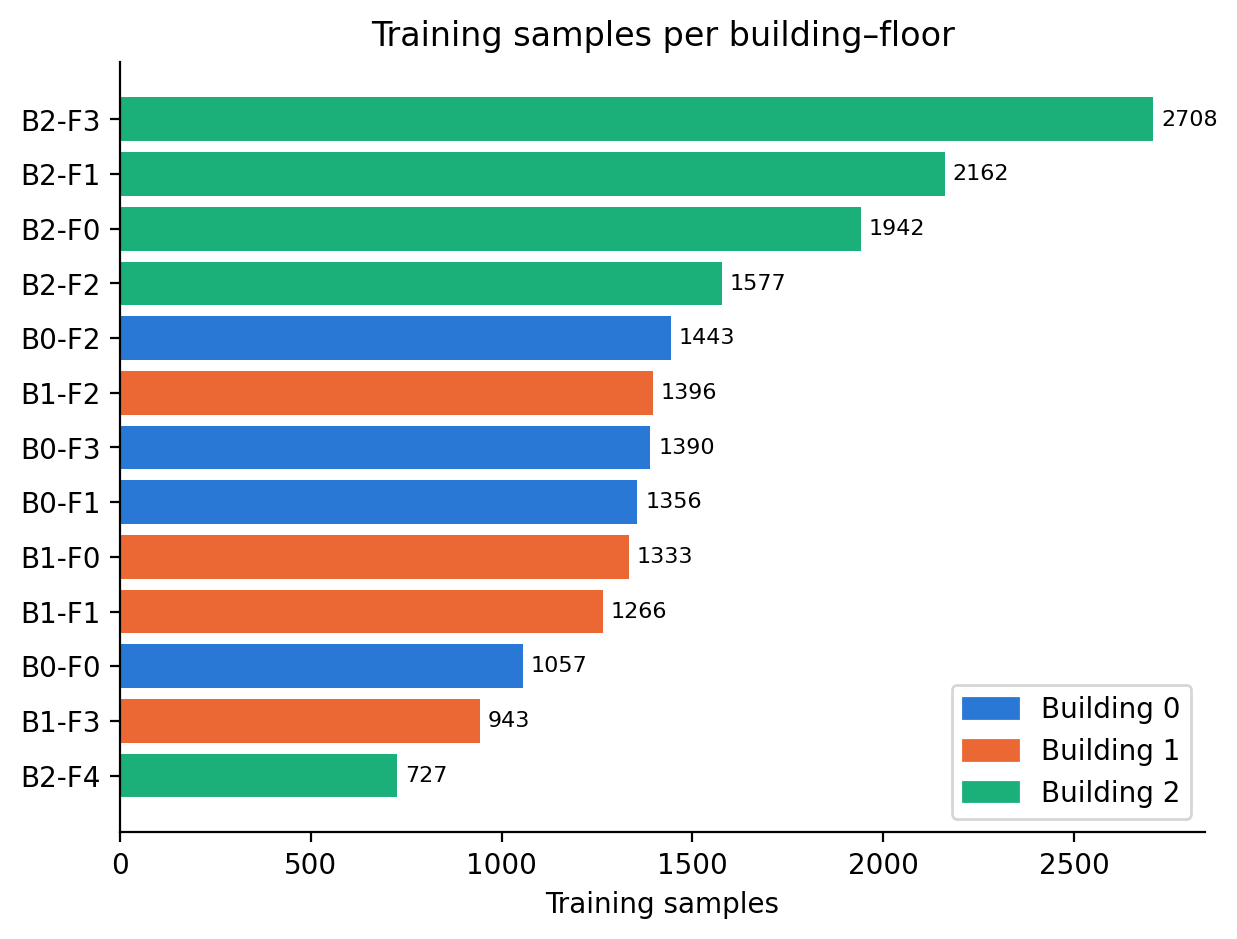
\includegraphics[width=0.9\columnwidth]{eda_building_floor_classes.png}
\caption{Training scans for each of the 13 building--floor combinations.}
\label{fig:classes}
\end{figure}

\subsection{Signal Characteristics}

The data is extremely sparse: 96.5\% of all signal values are ``not detected'', and a typical scan
picks up only 17 of the 520 access points. Among the real readings, most signals are weak, with a median
of $-82$~dBm in training and $-80$~dBm in validation (Fig.~\ref{fig:rssi}). Since the weakest real
reading is $-104$~dBm, the placeholder $+100$ should be replaced by a lower value such as $-110$~dBm,
which keeps the natural order ``not detected'' $<$ ``weakest detected''.

The number of detected access points also carries location information: scans in building~2 detect a
median of 19 access points, compared with 15--16 in buildings~0 and~1. This motivates aggregate
features for our models (number of detected access points and strongest signal per scan).

\begin{figure}[!t]
\centering
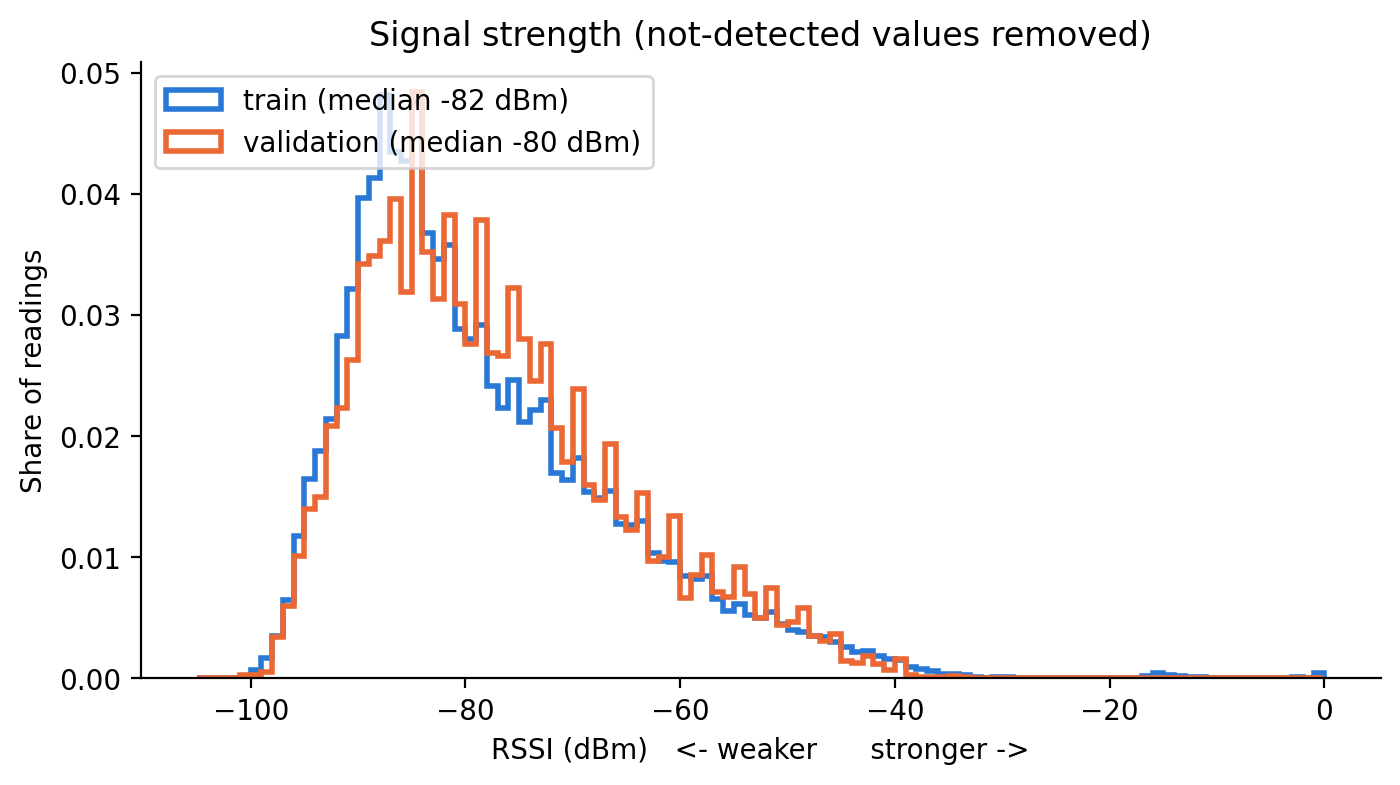
\includegraphics[width=\columnwidth]{eda_rssi_distribution.png}
\caption{Distribution of real RSSI readings (placeholder values removed).}
\label{fig:rssi}
\end{figure}

\subsection{Differences Between the Training and Validation Files}

The two files differ in several ways, so lower scores on the validation file than within the training
file are expected:
\begin{itemize}
\item \textbf{Time:} the files were collected 91 days apart, and each is dominated by a single session
(72.8\% of training scans on one day, 63\% of validation scans on another).
\item \textbf{Phones:} only 2 of the 11 phones in the validation file were used in training. Phones
differ by about 15~dB in typical reported signal strength and detect a median of 9 to 32 access points
per scan (Fig.~\ref{fig:phones}).
\item \textbf{Access points:} the detection rates of individual access points are only moderately
correlated between the files ($r = 0.65$), and 55 access points appear only in validation.
\item \textbf{Signal distributions:} a Kolmogorov--Smirnov test shows a moderate shift in the number of
access points per scan (KS $= 0.12$) and only small shifts in signal strength (KS $= 0.07$--$0.08$).
\end{itemize}

Despite these differences, the validation scans are well covered spatially: the median distance from a
validation scan to the nearest training position on the same floor is 0.9~m, and 90\% are within 4.6~m.
However, 35 validation scans (3.2\%) are more than 10~m from any training position, and we expect the
largest positioning errors there.

\begin{figure*}[!t]
\centering
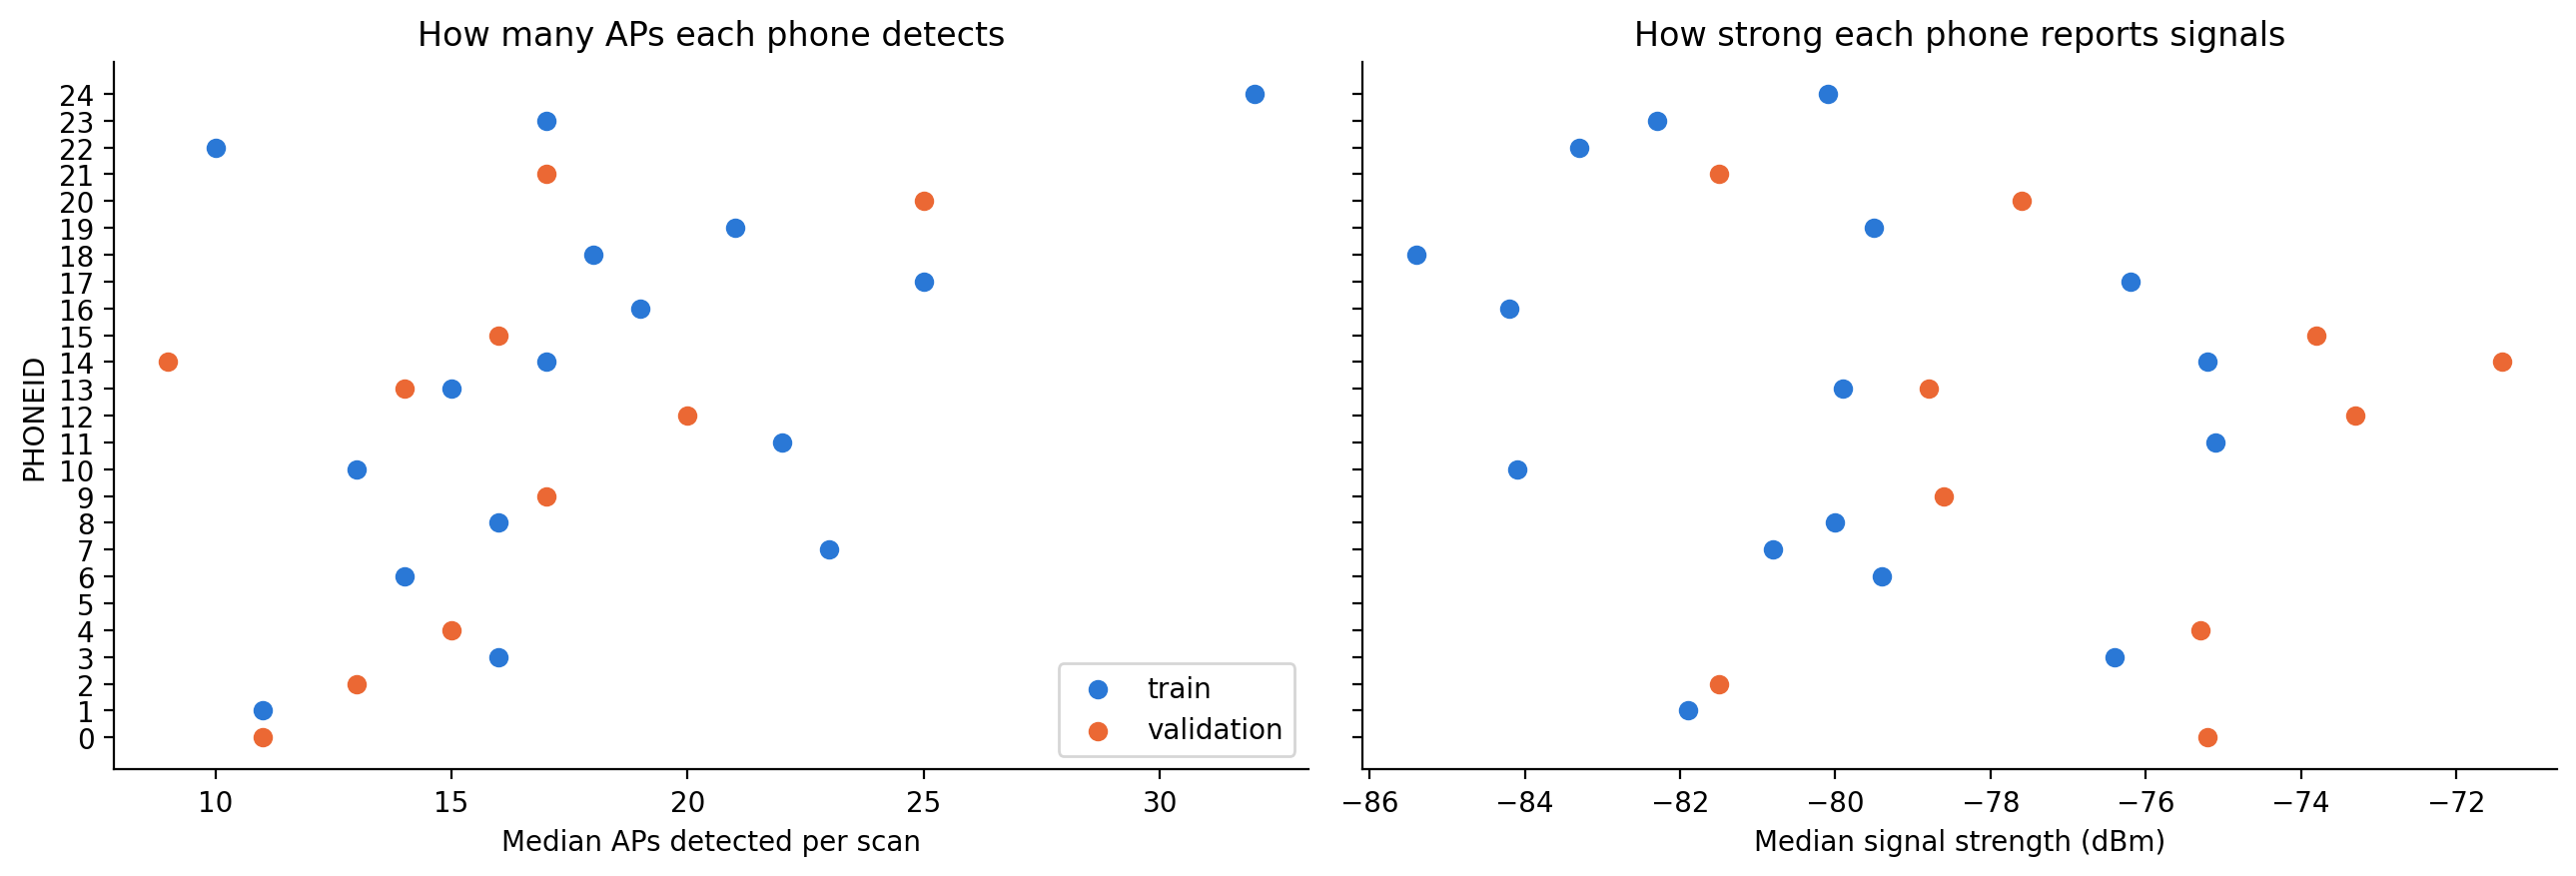
\includegraphics[width=0.85\textwidth]{eda_phone_differences.png}
\caption{Differences between phones (phones with at least 20 scans). Left: median number of access
points detected per scan. Right: median signal strength. Most validation phones (orange) were never
used in training.}
\label{fig:phones}
\end{figure*}

\subsection{Leakage Risks and Validation Strategy}

Each training position was scanned about 20 times, and each user collected only 1 to 8 of the 13
building--floor combinations using exactly one phone (Fig.~\ref{fig:users}). These properties determine
how models can be validated fairly. Table~\ref{tab:leakage} shows, for different 5-fold splits of the
training file, the share of test-fold scans whose exact position also appears in the training fold.

\begin{table}[!t]
\centering
\caption{Share of test-fold scans at a position already seen in training (5-fold splits of the training file)}
\label{tab:leakage}
\begin{tabular}{lr}
\toprule
\textbf{Split} & \textbf{Positions already seen} \\
\midrule
Random 5-fold & 100.0\% \\
Grouped by user & 78.2\% \\
Grouped by position & 0.0\% \\
\bottomrule
\end{tabular}
\end{table}

A random split places every test scan at a position the model has already seen, which would give
unrealistically optimistic scores. We therefore adopt the following protocol:
\begin{enumerate}
\item \textbf{Final results:} train on the training file and evaluate once on the validation file. No
validation scan is identical to a training scan, so this split has no direct leakage.
\item \textbf{Hyperparameter tuning:} 5-fold cross-validation within the training file, grouped by
position.
\item \textbf{Robustness:} 5-fold cross-validation grouped by user. Since each user used one phone, this
also tests generalisation to an unseen device.
\end{enumerate}
In addition, all preprocessing steps (placeholder replacement, scaling and column removal) are fitted on
the training file only, and the room-level columns \texttt{SPACEID} and \texttt{RELATIVEPOSITION} are
never used as inputs because they directly encode the location.

\begin{figure}[!t]
\centering
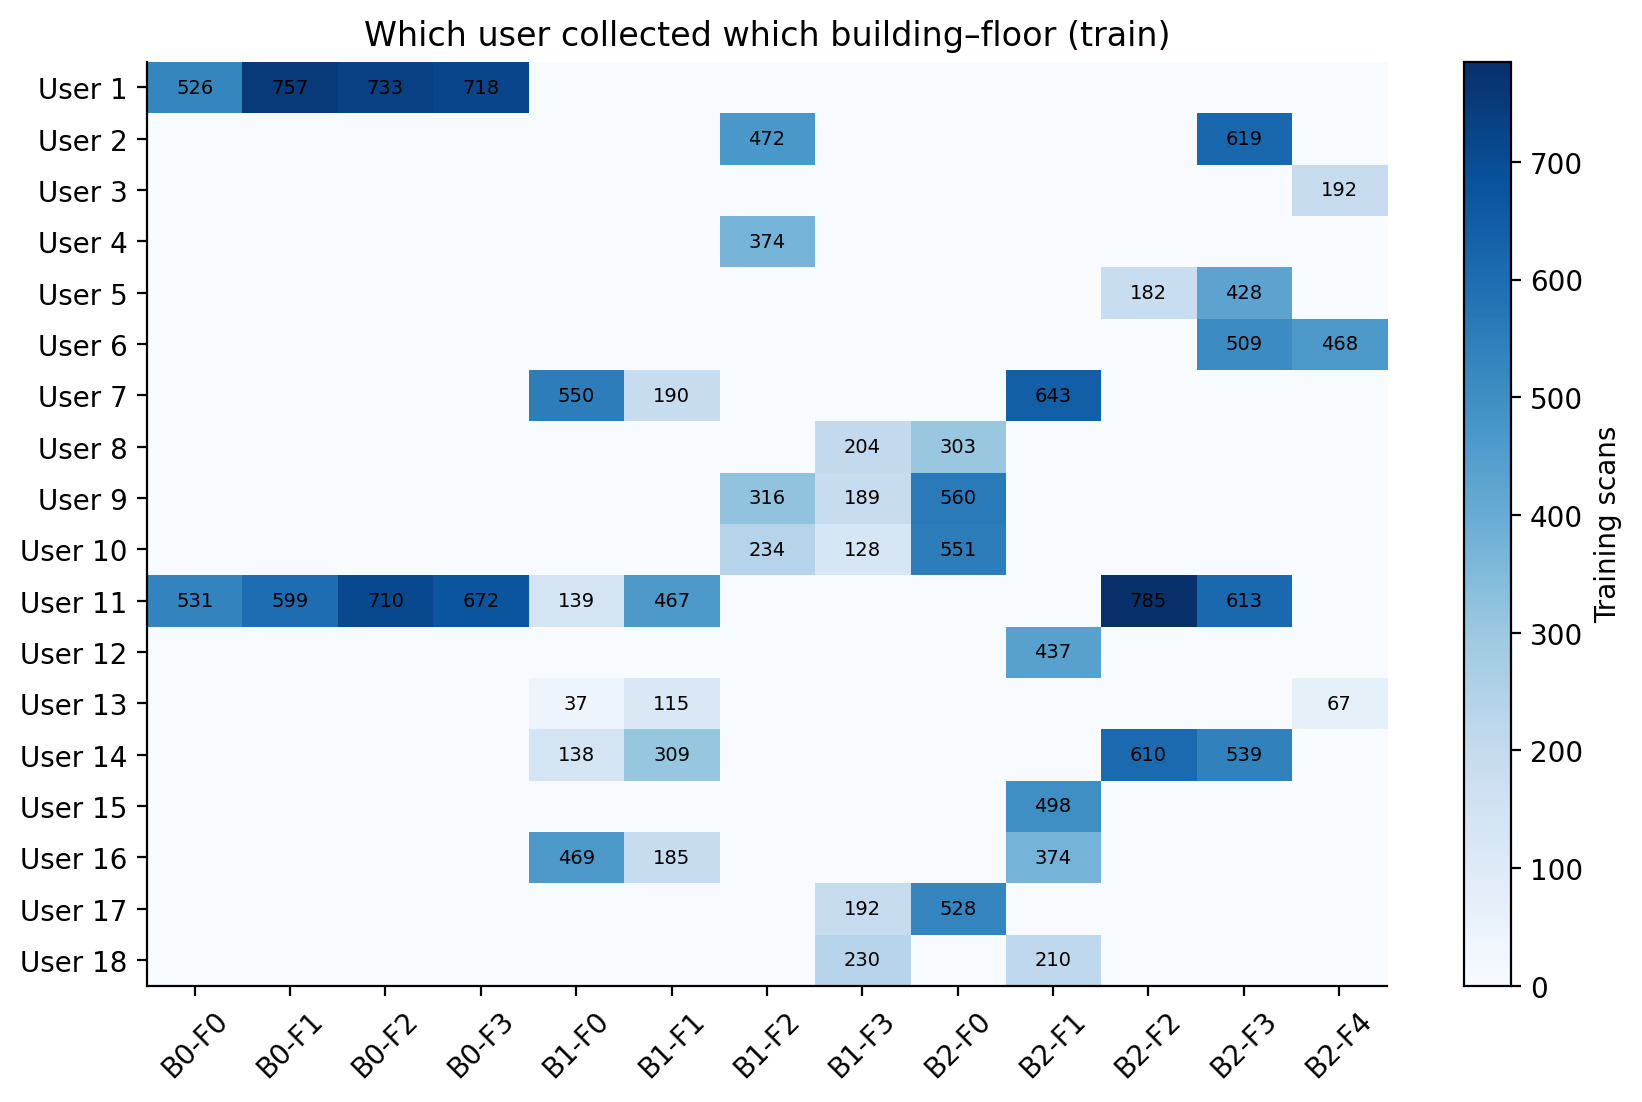
\includegraphics[width=\columnwidth]{eda_user_coverage.png}
\caption{Number of training scans collected by each user in each building--floor combination.}
\label{fig:users}
\end{figure}

% Figures are read from ../results/figures/ (see \graphicspath in main.tex)
% ---------------------------------------------------------------

\subsection{Dataset}

We use the UJIIndoorLoc dataset~\cite{torres2014ujiindoorloc, uci_ujiindoorloc}, a public benchmark for
Wi-Fi fingerprinting collected in three buildings of Universitat Jaume I, Spain. Each row is one Wi-Fi
scan taken by a smartphone. It contains the received signal strength (RSSI) of 520 wireless access
points (WAPs), the true location of the phone, and information about who took the scan, with which
phone, and when.

RSSI values are given in dBm and range from $-104$ (very weak) to $0$ (very strong). An access point
that was not detected is recorded as $+100$. This value is a placeholder, not a measurement, and it
must be handled explicitly because otherwise it would look like the strongest possible signal.

The prediction targets are the building (3 classes) and floor (5 classes), treated as classification,
and the longitude and latitude, treated as regression. The coordinates are projected positions in
metres, so positioning error can be reported in metres. The remaining columns (\texttt{SPACEID},
\texttt{RELATIVEPOSITION}, \texttt{USERID}, \texttt{PHONEID}, \texttt{TIMESTAMP}) are not used as model
inputs; we use them only for quality checks and to design fair validation splits.

The dataset is provided as two files: a training file and a validation file. The labels of the original
competition test set were never released, so, following common practice, we use the validation file
as our held-out test set and do not use it for any modelling decision. Table~\ref{tab:summary}
summarises both files.

\begin{table}[!t]
\centering
\caption{Summary of the two data files}
\label{tab:summary}
\begin{tabular}{lrr}
\toprule
 & \textbf{Train} & \textbf{Validation} \\
\midrule
Scans (rows) & 19{,}937 & 1{,}111 \\
Buildings / floors & 3 / 5 & 3 / 5 \\
Building--floor combinations & 13 & 13 \\
Users / phones & 18 / 16 & -- / 11 \\
Collection period & May--Jun 2013 & Sep--Oct 2013 \\
Signal values $=100$ (not detected) & 96.5\% & 96.8\% \\
Median APs detected per scan & 17 & 15 \\
Scans with no AP detected & 76 & 0 \\
Exact duplicate rows & 637 & 0 \\
Scans after removing duplicates & 19{,}300 & 1{,}111 \\
\bottomrule
\end{tabular}
\end{table}

\begin{figure}[!t]
\centering
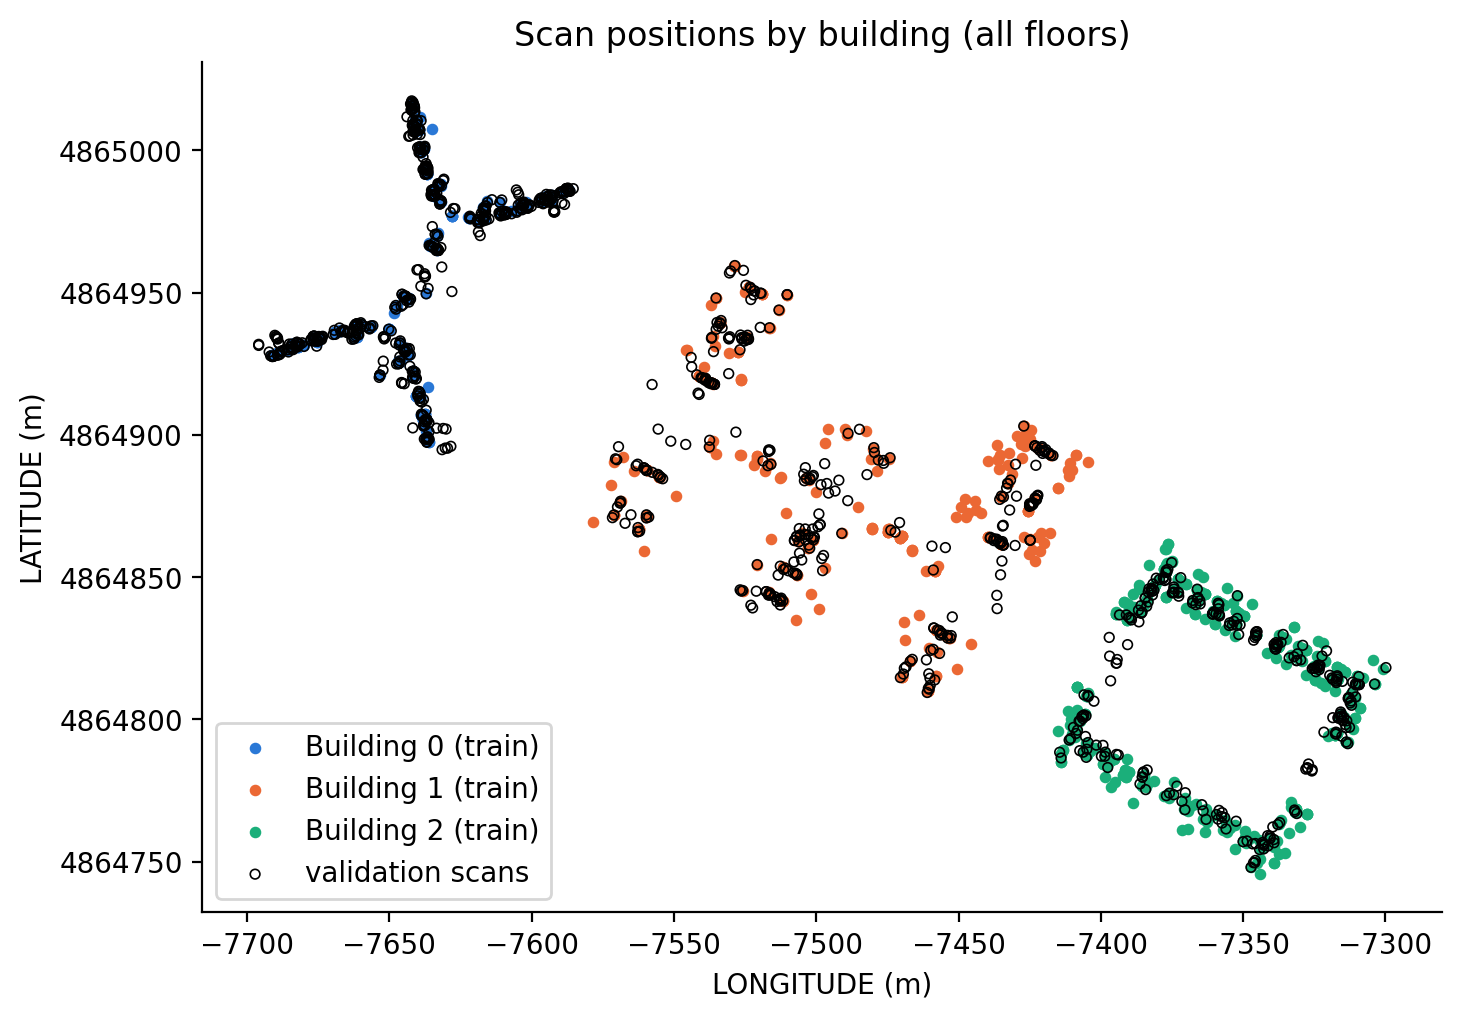
\includegraphics[width=\columnwidth]{eda_map_by_building.png}
\caption{Scan positions in the training file, coloured by building, with validation scans shown as
black circles. The three buildings occupy separate areas of the campus.}
\label{fig:map}
\end{figure}

\subsection{Data Quality}

Table~\ref{tab:quality} lists the quality checks and their outcome. The data is reliable overall: all
real RSSI values lie in the documented range, the labels are valid (floor~4 exists only in
building~2, the only five-floor building), and the three buildings are spatially separate
(Fig.~\ref{fig:map}).

A few issues require preprocessing decisions. First, the training file contains 637 exact duplicate
rows (3.2\%), 622 of them from a single user. None has conflicting labels, but copies falling on both
sides of a split would inflate validation scores, so we remove them. All results below use the remaining
19{,}300 training scans. Second, 73 of these scans detected no access point at all and therefore carry
no information; 59 of them come from a single user and phone, which points to a faulty recording
session. Third, 55 access points are never detected in the training file, so their columns are
constant and can be removed. The same 55 access points do appear in the validation file, while 153
access points seen in training never appear in validation, which shows that the Wi-Fi infrastructure
changed between the two collections.

Finally, 775 readings stronger than $-30$~dBm occur in 492 training scans, whereas the strongest
validation reading is $-34$~dBm. 87\% of these scans come from one device (phone~19), so we treat them
as a device artefact; capping readings at $-30$~dBm removes them.

\begin{table}[!t]
\centering
\caption{Data-quality checks on the training file}
\label{tab:quality}
\setlength{\tabcolsep}{3pt}
\begin{tabular}{p{0.27\columnwidth}p{0.40\columnwidth}p{0.27\columnwidth}}
\toprule
\textbf{Check} & \textbf{Result} & \textbf{Action} \\
\midrule
RSSI range & All real values in $[-104, 0]$ & None \\
Labels & Valid; floor 4 only in building 2 & None \\
Empty scans & 73 (59 from one device) & Remove \\
Duplicates & 637 exact duplicates (622 from one user) & Removed \\
Never-detected APs & 55 constant columns & Drop \\
Very strong readings & 492 scans, 87\% from phone 19 & Cap at $-30$ dBm \\
Validation metadata & User, room and position columns are always 0 & Never use as inputs \\
\bottomrule
\end{tabular}
\end{table}

\subsection{Label Distributions}

Fig.~\ref{fig:buildings} shows that the two files emphasise different buildings: building~2 makes up
47.2\% of the training scans, while building~0 makes up 48.2\% of the validation scans. Overall
validation accuracy is therefore driven mostly by building~0, and we report results per building as
well as overall.

Class imbalance is moderate (Fig.~\ref{fig:classes}). Every building--floor combination has at least
727 training scans, recorded at 50--113 distinct positions with about 20 scans per position. The
largest combination (building~2, floor~3) has 3.7 times as many scans as the smallest (building~2,
floor~4). A classifier that always predicts the most frequent class would reach 47.2\% building
accuracy and 26.1\% floor accuracy; these are the baselines any model must clearly exceed. Because of
the imbalance, we report macro-F1 alongside accuracy.

\begin{figure}[!t]
\centering
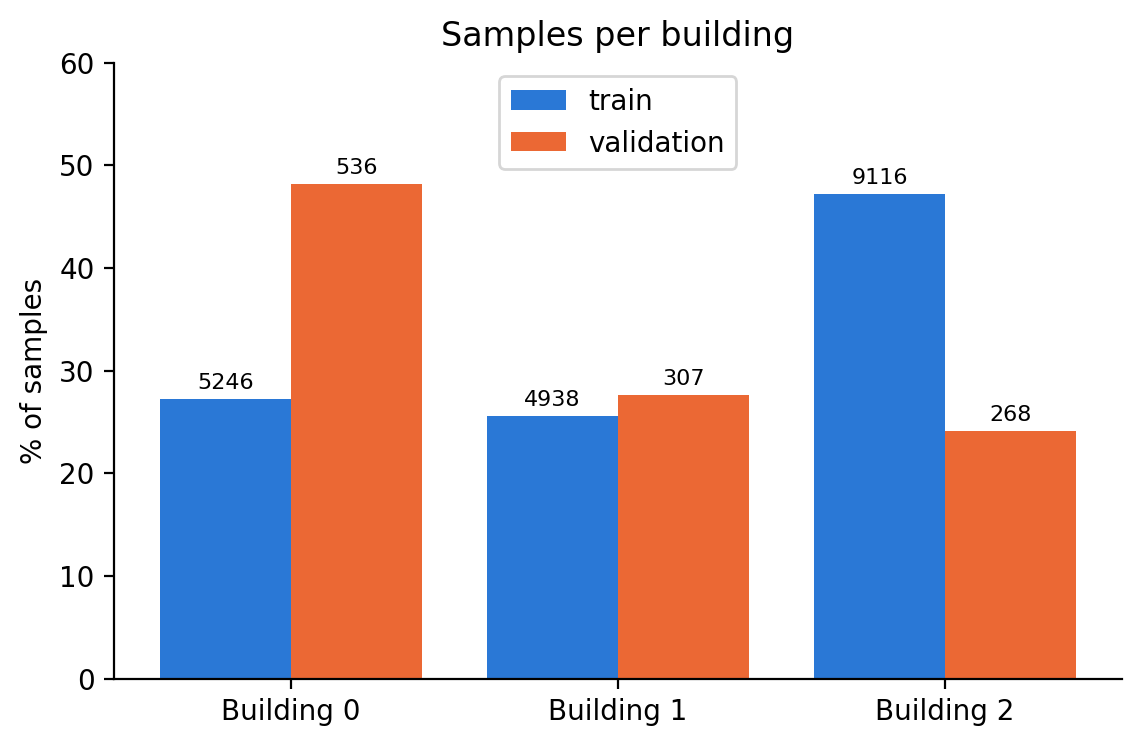
\includegraphics[width=0.9\columnwidth]{eda_samples_per_building.png}
\caption{Share of scans per building in each file (counts above the bars).}
\label{fig:buildings}
\end{figure}

\begin{figure}[!t]
\centering
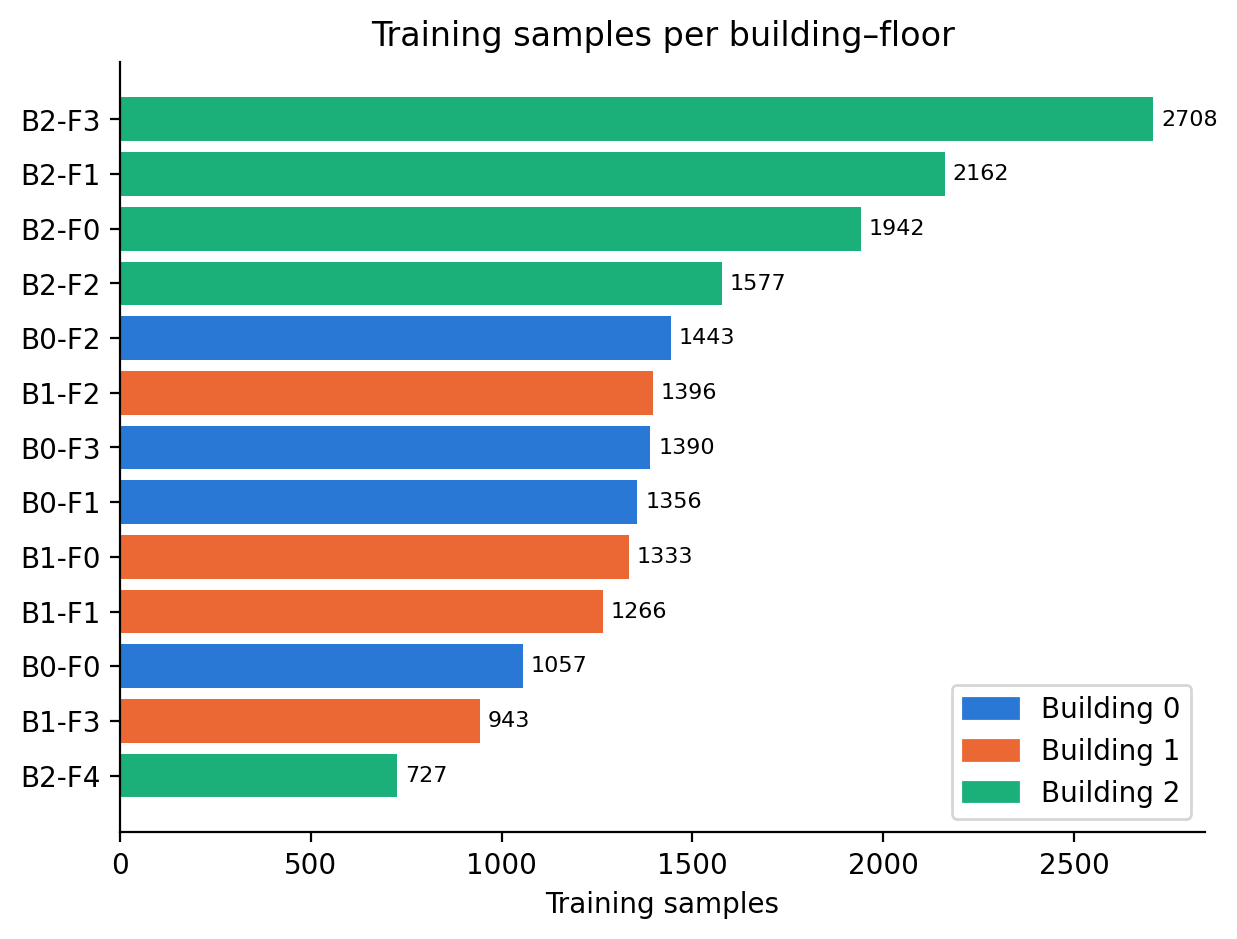
\includegraphics[width=0.9\columnwidth]{eda_building_floor_classes.png}
\caption{Training scans for each of the 13 building--floor combinations.}
\label{fig:classes}
\end{figure}

\subsection{Signal Characteristics}

The data is extremely sparse: 96.5\% of all signal values are ``not detected'', and a typical scan
picks up only 17 of the 520 access points. Among the real readings, most signals are weak, with a median
of $-82$~dBm in training and $-80$~dBm in validation (Fig.~\ref{fig:rssi}). Since the weakest real
reading is $-104$~dBm, the placeholder $+100$ should be replaced by a lower value such as $-110$~dBm,
which keeps the natural order ``not detected'' $<$ ``weakest detected''.

The number of detected access points also carries location information: scans in building~2 detect a
median of 19 access points, compared with 15--16 in buildings~0 and~1. This motivates aggregate
features for our models (number of detected access points and strongest signal per scan).

\begin{figure}[!t]
\centering
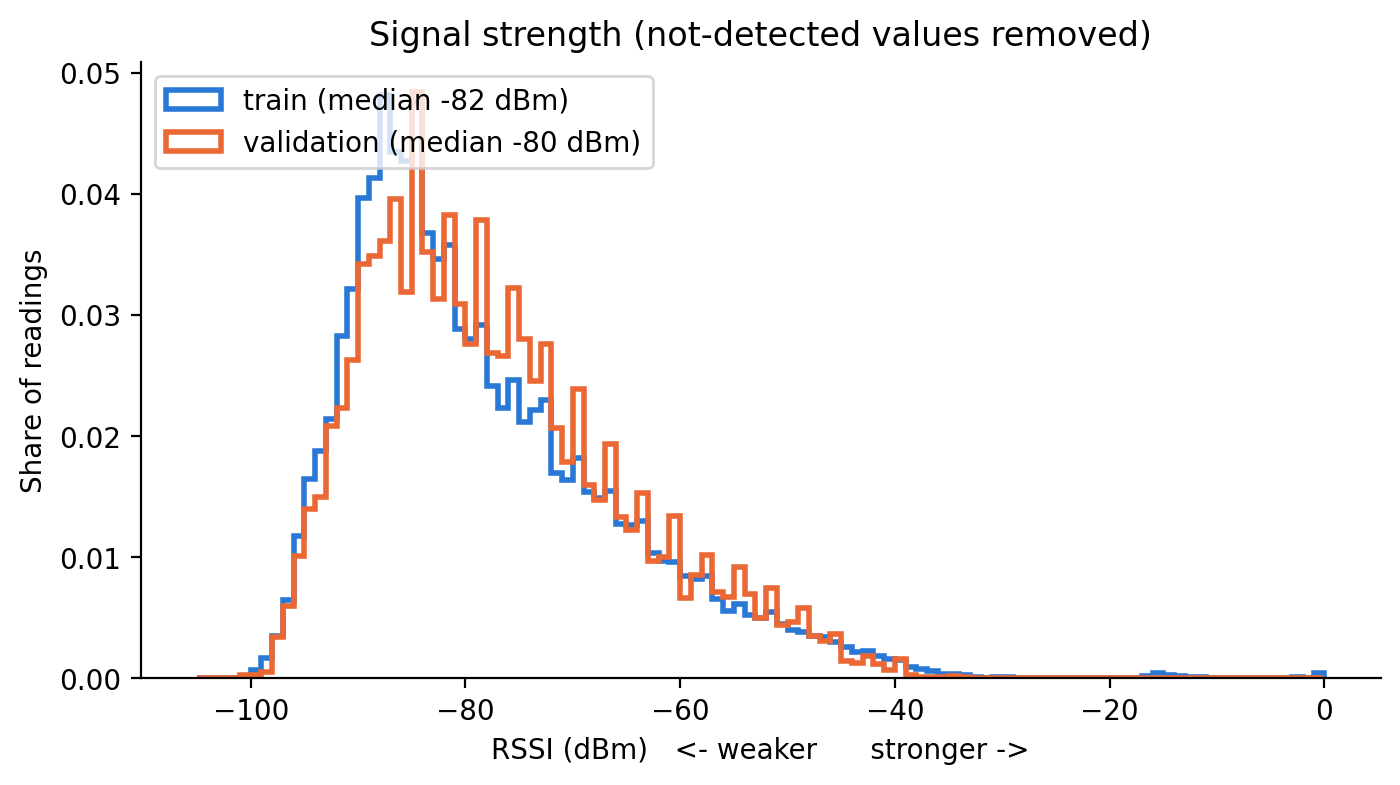
\includegraphics[width=\columnwidth]{eda_rssi_distribution.png}
\caption{Distribution of real RSSI readings (placeholder values removed).}
\label{fig:rssi}
\end{figure}

\subsection{Differences Between the Training and Validation Files}

The two files differ in several ways, so lower scores on the validation file than within the training
file are expected:
\begin{itemize}
\item \textbf{Time:} the files were collected 91 days apart, and each is dominated by a single session
(72.8\% of training scans on one day, 63\% of validation scans on another).
\item \textbf{Phones:} only 2 of the 11 phones in the validation file were used in training. Phones
differ by about 15~dB in typical reported signal strength and detect a median of 9 to 32 access points
per scan (Fig.~\ref{fig:phones}).
\item \textbf{Access points:} the detection rates of individual access points are only moderately
correlated between the files ($r = 0.65$), and 55 access points appear only in validation.
\item \textbf{Signal distributions:} a Kolmogorov--Smirnov test shows a moderate shift in the number of
access points per scan (KS $= 0.12$) and only small shifts in signal strength (KS $= 0.07$--$0.08$).
\end{itemize}

Despite these differences, the validation scans are well covered spatially: the median distance from a
validation scan to the nearest training position on the same floor is 0.9~m, and 90\% are within 4.6~m.
However, 35 validation scans (3.2\%) are more than 10~m from any training position, and we expect the
largest positioning errors there.

\begin{figure*}[!t]
\centering
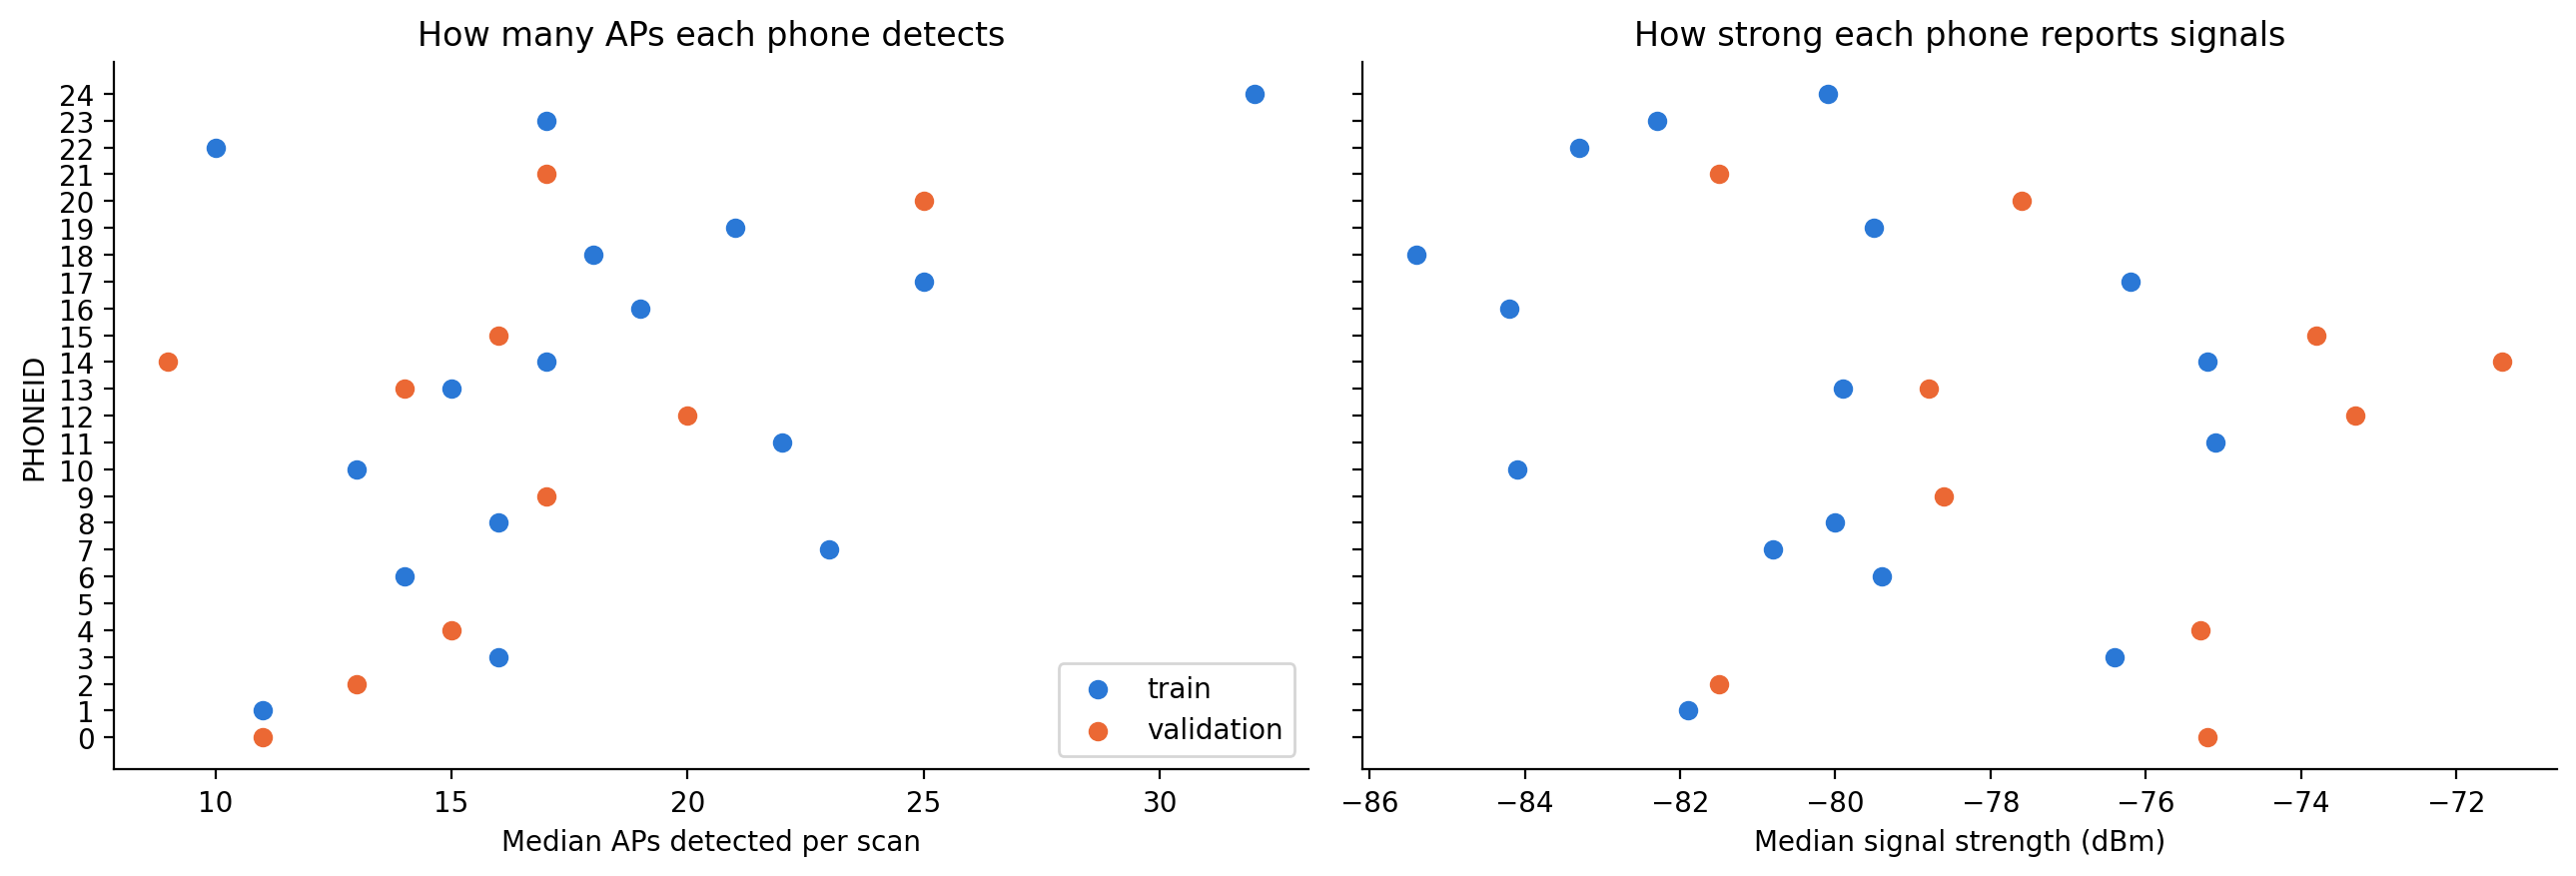
\includegraphics[width=0.85\textwidth]{eda_phone_differences.png}
\caption{Differences between phones (phones with at least 20 scans). Left: median number of access
points detected per scan. Right: median signal strength. Most validation phones (orange) were never
used in training.}
\label{fig:phones}
\end{figure*}

\subsection{Leakage Risks and Validation Strategy}

Each training position was scanned about 20 times, and each user collected only 1 to 8 of the 13
building--floor combinations using exactly one phone (Fig.~\ref{fig:users}). These properties determine
how models can be validated fairly. Table~\ref{tab:leakage} shows, for different 5-fold splits of the
training file, the share of test-fold scans whose exact position also appears in the training fold.

\begin{table}[!t]
\centering
\caption{Share of test-fold scans at a position already seen in training (5-fold splits of the training file)}
\label{tab:leakage}
\begin{tabular}{lr}
\toprule
\textbf{Split} & \textbf{Positions already seen} \\
\midrule
Random 5-fold & 100.0\% \\
Grouped by user & 78.2\% \\
Grouped by position & 0.0\% \\
\bottomrule
\end{tabular}
\end{table}

A random split places every test scan at a position the model has already seen, which would give
unrealistically optimistic scores. We therefore adopt the following protocol:
\begin{enumerate}
\item \textbf{Final results:} train on the training file and evaluate once on the validation file. No
validation scan is identical to a training scan, so this split has no direct leakage.
\item \textbf{Hyperparameter tuning:} 5-fold cross-validation within the training file, grouped by
position.
\item \textbf{Robustness:} 5-fold cross-validation grouped by user. Since each user used one phone, this
also tests generalisation to an unseen device.
\end{enumerate}
In addition, all preprocessing steps (placeholder replacement, scaling and column removal) are fitted on
the training file only, and the room-level columns \texttt{SPACEID} and \texttt{RELATIVEPOSITION} are
never used as inputs because they directly encode the location.

\begin{figure}[!t]
\centering
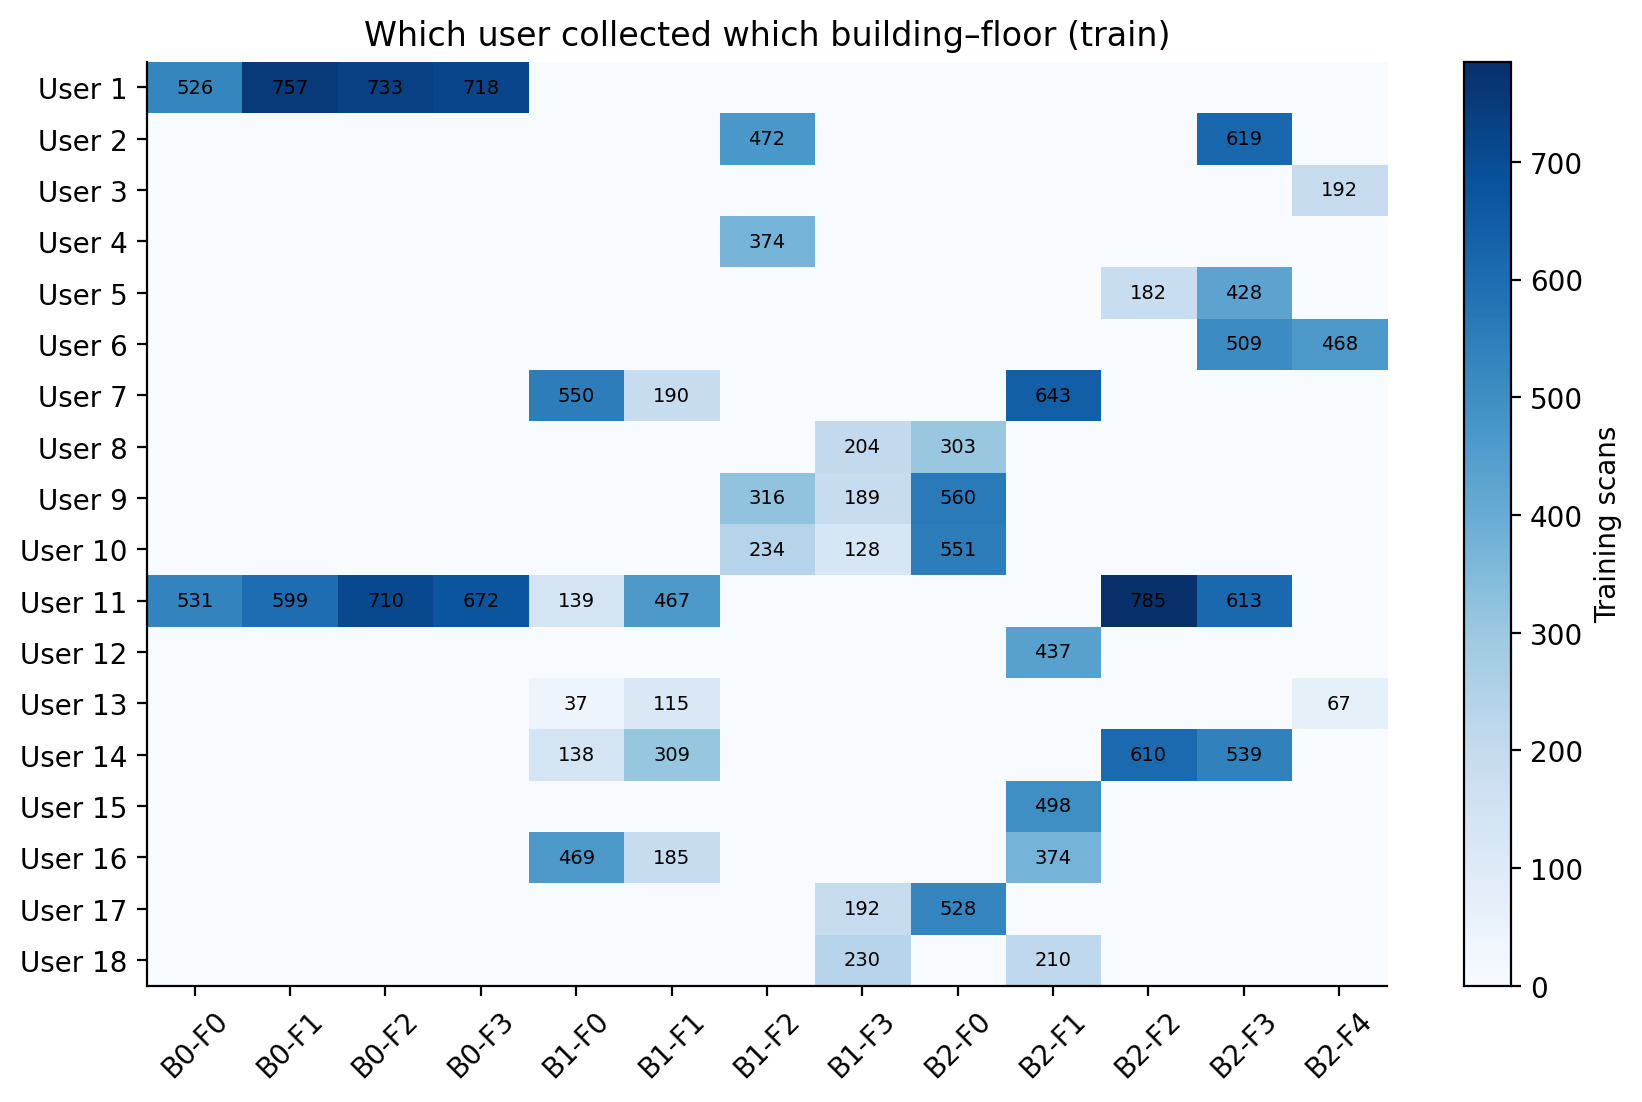
\includegraphics[width=\columnwidth]{eda_user_coverage.png}
\caption{Number of training scans collected by each user in each building--floor combination.}
\label{fig:users}
\end{figure}

% Figures are read from ../results/figures/ (see \graphicspath in main.tex)
% ---------------------------------------------------------------

\subsection{Dataset}

We use the UJIIndoorLoc dataset~\cite{torres2014ujiindoorloc, uci_ujiindoorloc}, a public benchmark for
Wi-Fi fingerprinting collected in three buildings of Universitat Jaume I, Spain. Each row is one Wi-Fi
scan taken by a smartphone. It contains the received signal strength (RSSI) of 520 wireless access
points (WAPs), the true location of the phone, and information about who took the scan, with which
phone, and when.

RSSI values are given in dBm and range from $-104$ (very weak) to $0$ (very strong). An access point
that was not detected is recorded as $+100$. This value is a placeholder, not a measurement, and it
must be handled explicitly because otherwise it would look like the strongest possible signal.

The prediction targets are the building (3 classes) and floor (5 classes), treated as classification,
and the longitude and latitude, treated as regression. The coordinates are projected positions in
metres, so positioning error can be reported in metres. The remaining columns (\texttt{SPACEID},
\texttt{RELATIVEPOSITION}, \texttt{USERID}, \texttt{PHONEID}, \texttt{TIMESTAMP}) are not used as model
inputs; we use them only for quality checks and to design fair validation splits.

The dataset is provided as two files: a training file and a validation file. The labels of the original
competition test set were never released, so, following common practice, we use the validation file
as our held-out test set and do not use it for any modelling decision. Table~\ref{tab:summary}
summarises both files.

\begin{table}[!t]
\centering
\caption{Summary of the two data files}
\label{tab:summary}
\begin{tabular}{lrr}
\toprule
 & \textbf{Train} & \textbf{Validation} \\
\midrule
Scans (rows) & 19{,}937 & 1{,}111 \\
Buildings / floors & 3 / 5 & 3 / 5 \\
Building--floor combinations & 13 & 13 \\
Users / phones & 18 / 16 & -- / 11 \\
Collection period & May--Jun 2013 & Sep--Oct 2013 \\
Signal values $=100$ (not detected) & 96.5\% & 96.8\% \\
Median APs detected per scan & 17 & 15 \\
Scans with no AP detected & 76 & 0 \\
Exact duplicate rows & 637 & 0 \\
Scans after removing duplicates & 19{,}300 & 1{,}111 \\
\bottomrule
\end{tabular}
\end{table}

\begin{figure}[!t]
\centering
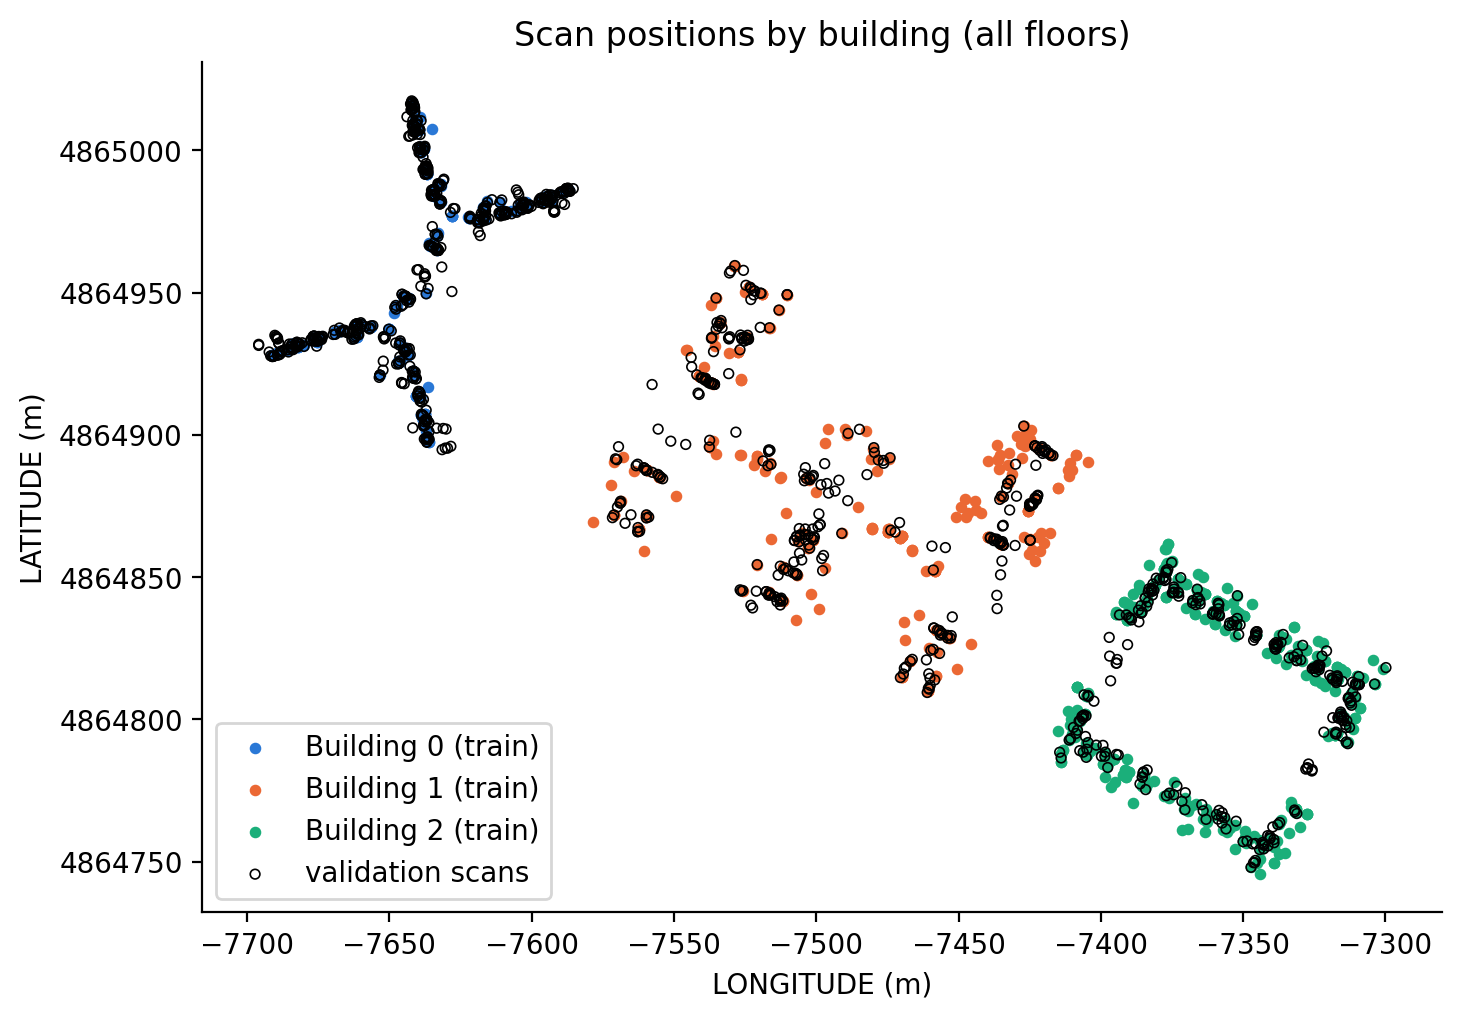
\includegraphics[width=\columnwidth]{eda_map_by_building.png}
\caption{Scan positions in the training file, coloured by building, with validation scans shown as
black circles. The three buildings occupy separate areas of the campus.}
\label{fig:map}
\end{figure}

\subsection{Data Quality}

Table~\ref{tab:quality} lists the quality checks and their outcome. The data is reliable overall: all
real RSSI values lie in the documented range, the labels are valid (floor~4 exists only in
building~2, the only five-floor building), and the three buildings are spatially separate
(Fig.~\ref{fig:map}).

A few issues require preprocessing decisions. First, the training file contains 637 exact duplicate
rows (3.2\%), 622 of them from a single user. None has conflicting labels, but copies falling on both
sides of a split would inflate validation scores, so we remove them. All results below use the remaining
19{,}300 training scans. Second, 73 of these scans detected no access point at all and therefore carry
no information; 59 of them come from a single user and phone, which points to a faulty recording
session. Third, 55 access points are never detected in the training file, so their columns are
constant and can be removed. The same 55 access points do appear in the validation file, while 153
access points seen in training never appear in validation, which shows that the Wi-Fi infrastructure
changed between the two collections.

Finally, 775 readings stronger than $-30$~dBm occur in 492 training scans, whereas the strongest
validation reading is $-34$~dBm. 87\% of these scans come from one device (phone~19), so we treat them
as a device artefact; capping readings at $-30$~dBm removes them.

\begin{table}[!t]
\centering
\caption{Data-quality checks on the training file}
\label{tab:quality}
\setlength{\tabcolsep}{3pt}
\begin{tabular}{p{0.27\columnwidth}p{0.40\columnwidth}p{0.27\columnwidth}}
\toprule
\textbf{Check} & \textbf{Result} & \textbf{Action} \\
\midrule
RSSI range & All real values in $[-104, 0]$ & None \\
Labels & Valid; floor 4 only in building 2 & None \\
Empty scans & 73 (59 from one device) & Remove \\
Duplicates & 637 exact duplicates (622 from one user) & Removed \\
Never-detected APs & 55 constant columns & Drop \\
Very strong readings & 492 scans, 87\% from phone 19 & Cap at $-30$ dBm \\
Validation metadata & User, room and position columns are always 0 & Never use as inputs \\
\bottomrule
\end{tabular}
\end{table}

\subsection{Label Distributions}

Fig.~\ref{fig:buildings} shows that the two files emphasise different buildings: building~2 makes up
47.2\% of the training scans, while building~0 makes up 48.2\% of the validation scans. Overall
validation accuracy is therefore driven mostly by building~0, and we report results per building as
well as overall.

Class imbalance is moderate (Fig.~\ref{fig:classes}). Every building--floor combination has at least
727 training scans, recorded at 50--113 distinct positions with about 20 scans per position. The
largest combination (building~2, floor~3) has 3.7 times as many scans as the smallest (building~2,
floor~4). A classifier that always predicts the most frequent class would reach 47.2\% building
accuracy and 26.1\% floor accuracy; these are the baselines any model must clearly exceed. Because of
the imbalance, we report macro-F1 alongside accuracy.

\begin{figure}[!t]
\centering
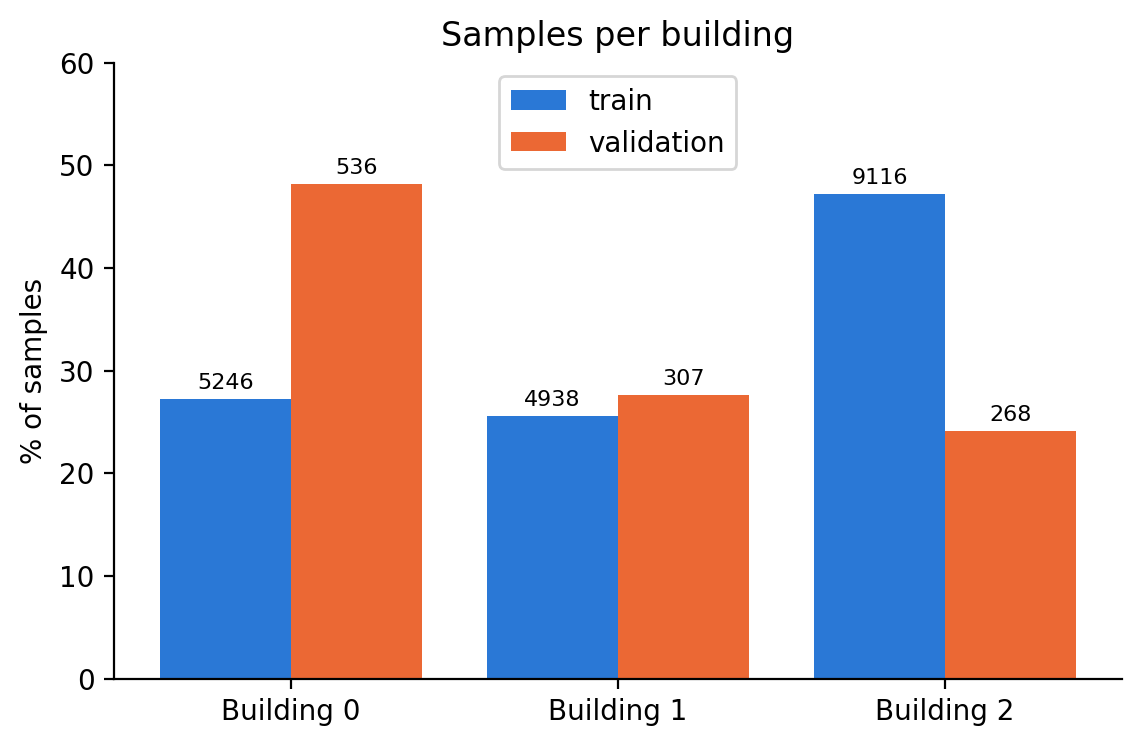
\includegraphics[width=0.9\columnwidth]{eda_samples_per_building.png}
\caption{Share of scans per building in each file (counts above the bars).}
\label{fig:buildings}
\end{figure}

\begin{figure}[!t]
\centering
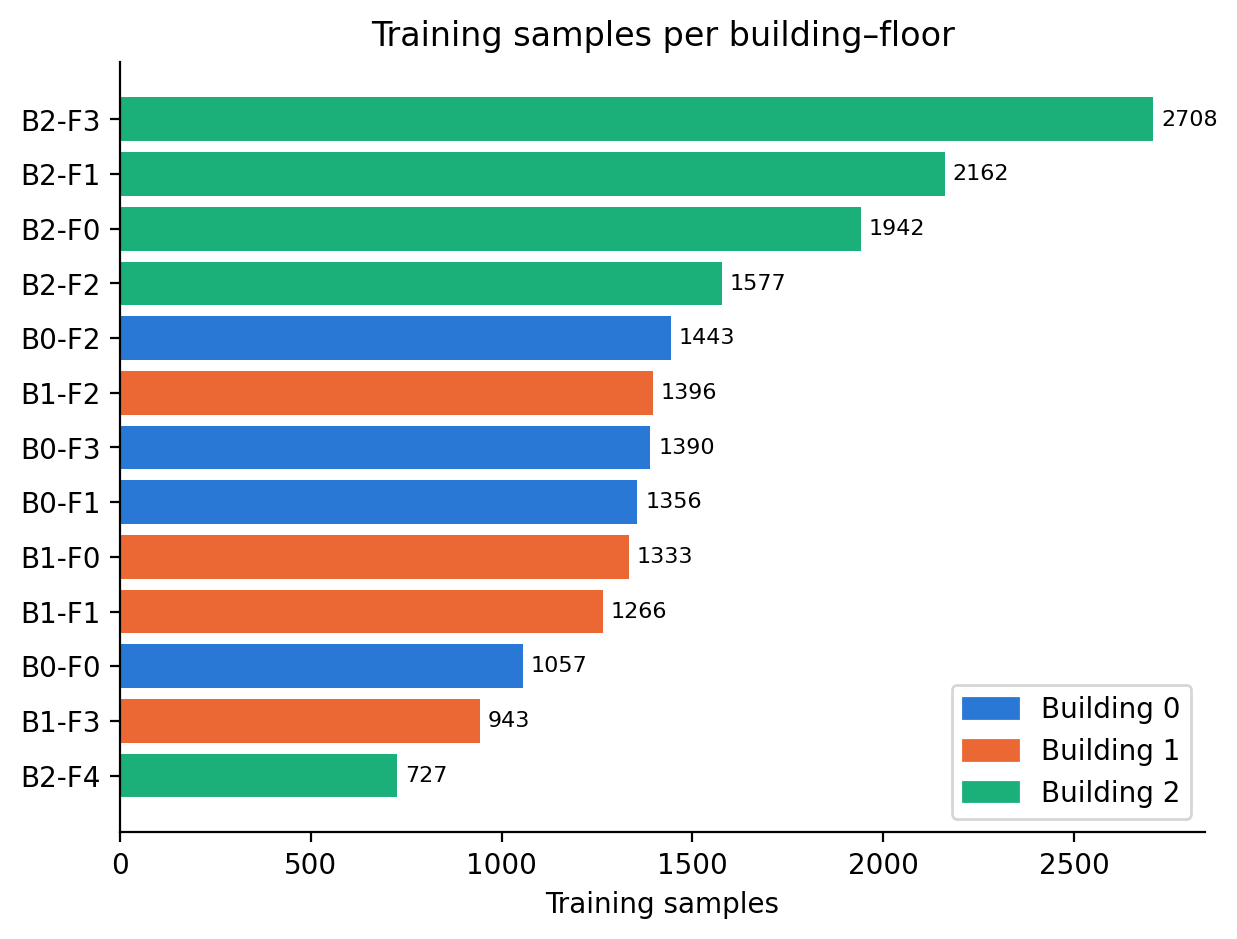
\includegraphics[width=0.9\columnwidth]{eda_building_floor_classes.png}
\caption{Training scans for each of the 13 building--floor combinations.}
\label{fig:classes}
\end{figure}

\subsection{Signal Characteristics}

The data is extremely sparse: 96.5\% of all signal values are ``not detected'', and a typical scan
picks up only 17 of the 520 access points. Among the real readings, most signals are weak, with a median
of $-82$~dBm in training and $-80$~dBm in validation (Fig.~\ref{fig:rssi}). Since the weakest real
reading is $-104$~dBm, the placeholder $+100$ should be replaced by a lower value such as $-110$~dBm,
which keeps the natural order ``not detected'' $<$ ``weakest detected''.

The number of detected access points also carries location information: scans in building~2 detect a
median of 19 access points, compared with 15--16 in buildings~0 and~1. This motivates aggregate
features for our models (number of detected access points and strongest signal per scan).

\begin{figure}[!t]
\centering
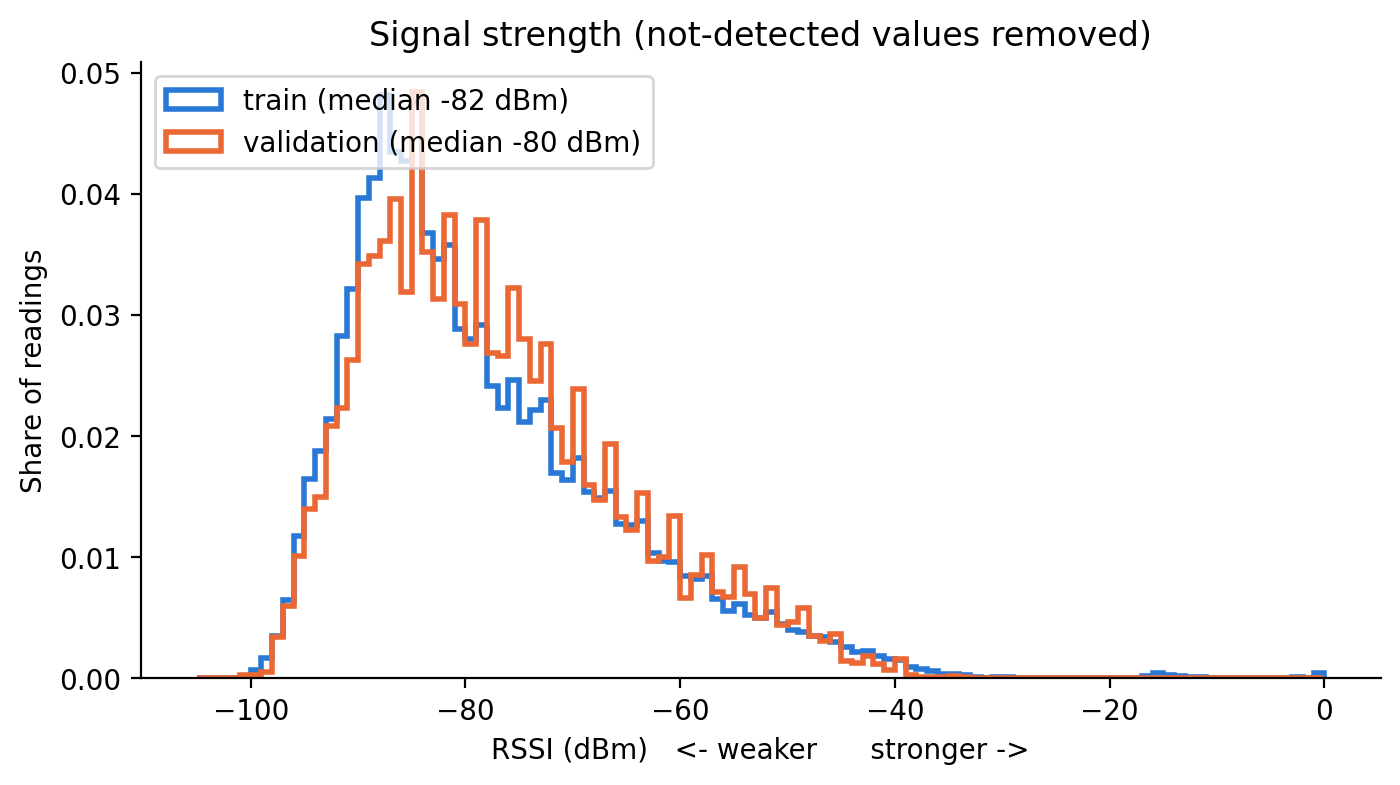
\includegraphics[width=\columnwidth]{eda_rssi_distribution.png}
\caption{Distribution of real RSSI readings (placeholder values removed).}
\label{fig:rssi}
\end{figure}

\subsection{Differences Between the Training and Validation Files}

The two files differ in several ways, so lower scores on the validation file than within the training
file are expected:
\begin{itemize}
\item \textbf{Time:} the files were collected 91 days apart, and each is dominated by a single session
(72.8\% of training scans on one day, 63\% of validation scans on another).
\item \textbf{Phones:} only 2 of the 11 phones in the validation file were used in training. Phones
differ by about 15~dB in typical reported signal strength and detect a median of 9 to 32 access points
per scan (Fig.~\ref{fig:phones}).
\item \textbf{Access points:} the detection rates of individual access points are only moderately
correlated between the files ($r = 0.65$), and 55 access points appear only in validation.
\item \textbf{Signal distributions:} a Kolmogorov--Smirnov test shows a moderate shift in the number of
access points per scan (KS $= 0.12$) and only small shifts in signal strength (KS $= 0.07$--$0.08$).
\end{itemize}

Despite these differences, the validation scans are well covered spatially: the median distance from a
validation scan to the nearest training position on the same floor is 0.9~m, and 90\% are within 4.6~m.
However, 35 validation scans (3.2\%) are more than 10~m from any training position, and we expect the
largest positioning errors there.

\begin{figure*}[!t]
\centering
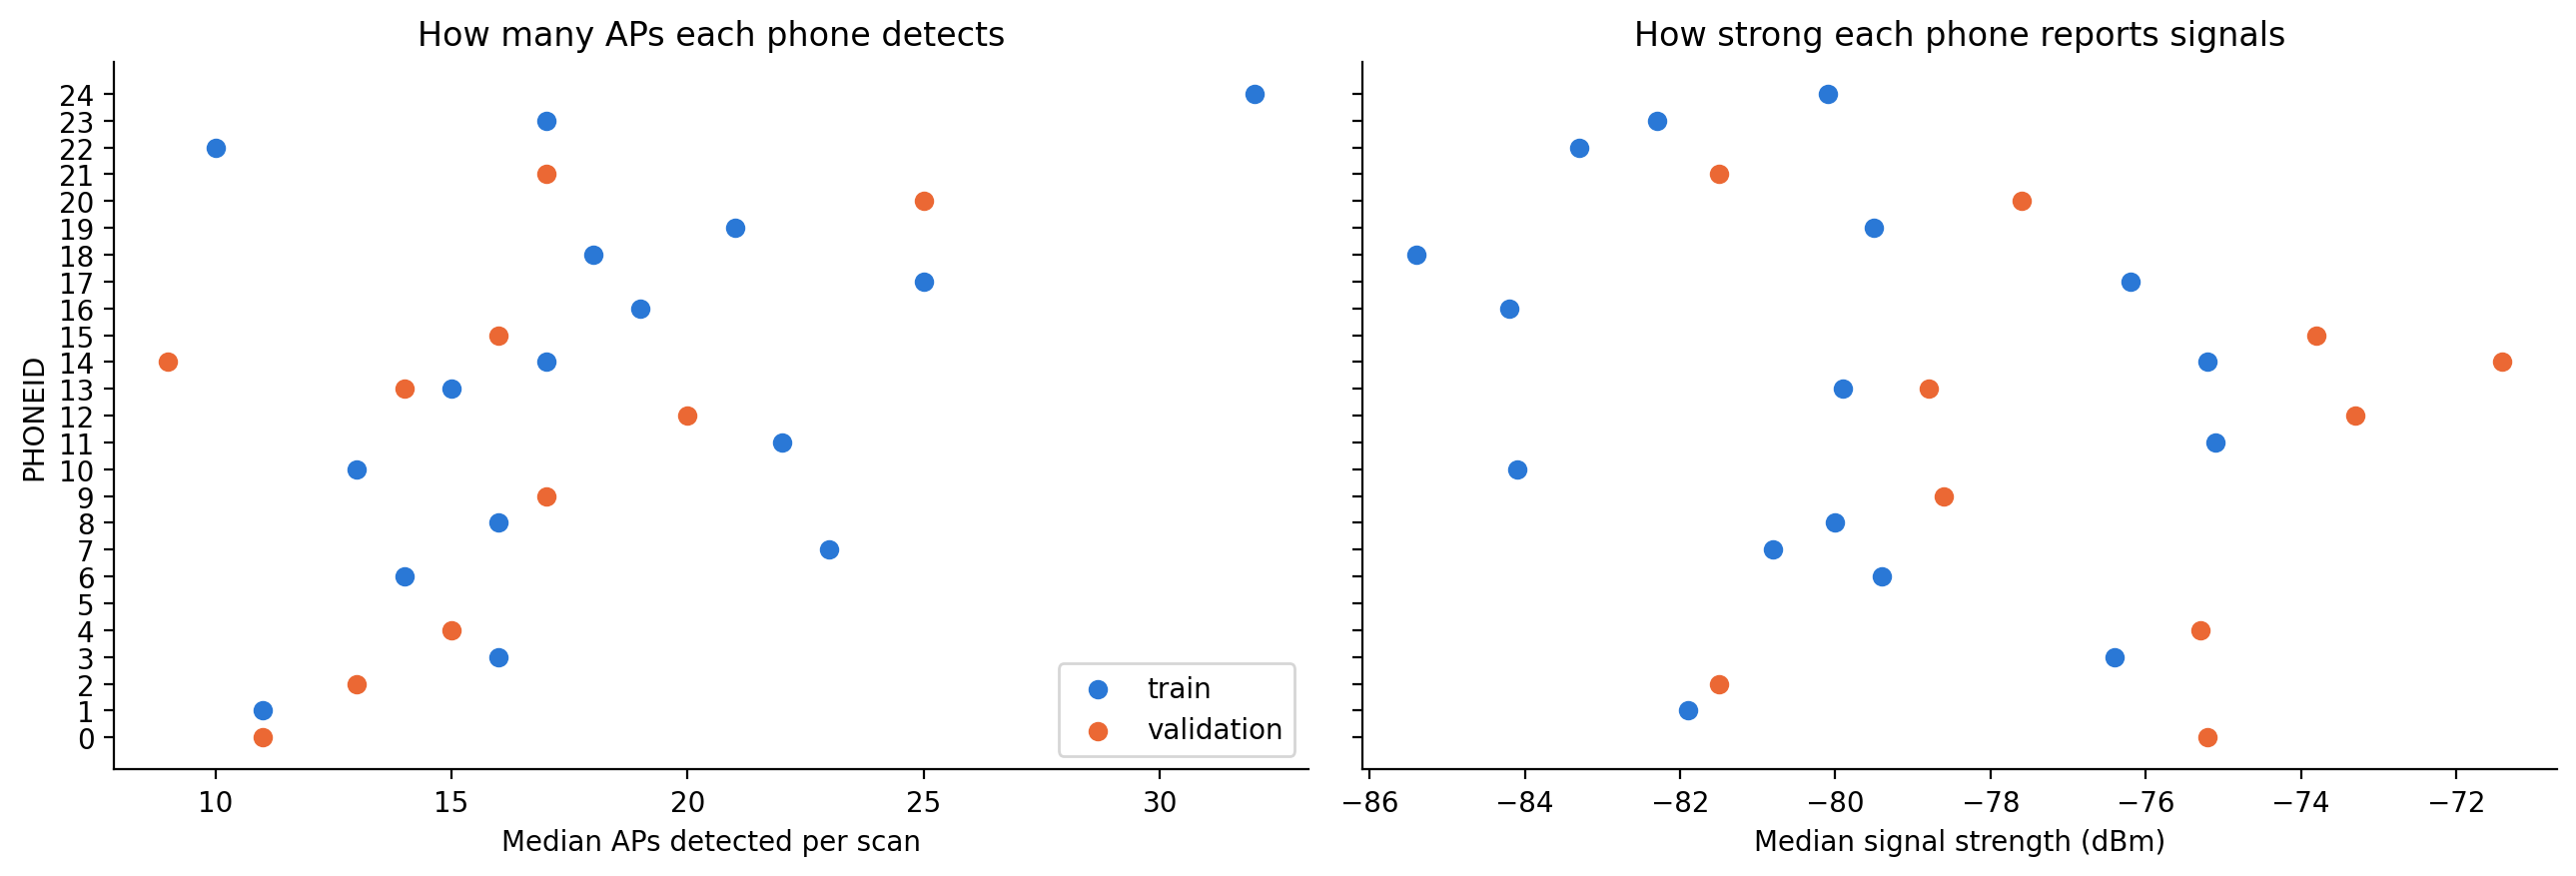
\includegraphics[width=0.85\textwidth]{eda_phone_differences.png}
\caption{Differences between phones (phones with at least 20 scans). Left: median number of access
points detected per scan. Right: median signal strength. Most validation phones (orange) were never
used in training.}
\label{fig:phones}
\end{figure*}

\subsection{Leakage Risks and Validation Strategy}

Each training position was scanned about 20 times, and each user collected only 1 to 8 of the 13
building--floor combinations using exactly one phone (Fig.~\ref{fig:users}). These properties determine
how models can be validated fairly. Table~\ref{tab:leakage} shows, for different 5-fold splits of the
training file, the share of test-fold scans whose exact position also appears in the training fold.

\begin{table}[!t]
\centering
\caption{Share of test-fold scans at a position already seen in training (5-fold splits of the training file)}
\label{tab:leakage}
\begin{tabular}{lr}
\toprule
\textbf{Split} & \textbf{Positions already seen} \\
\midrule
Random 5-fold & 100.0\% \\
Grouped by user & 78.2\% \\
Grouped by position & 0.0\% \\
\bottomrule
\end{tabular}
\end{table}

A random split places every test scan at a position the model has already seen, which would give
unrealistically optimistic scores. We therefore adopt the following protocol:
\begin{enumerate}
\item \textbf{Final results:} train on the training file and evaluate once on the validation file. No
validation scan is identical to a training scan, so this split has no direct leakage.
\item \textbf{Hyperparameter tuning:} 5-fold cross-validation within the training file, grouped by
position.
\item \textbf{Robustness:} 5-fold cross-validation grouped by user. Since each user used one phone, this
also tests generalisation to an unseen device.
\end{enumerate}
In addition, all preprocessing steps (placeholder replacement, scaling and column removal) are fitted on
the training file only, and the room-level columns \texttt{SPACEID} and \texttt{RELATIVEPOSITION} are
never used as inputs because they directly encode the location.

\begin{figure}[!t]
\centering
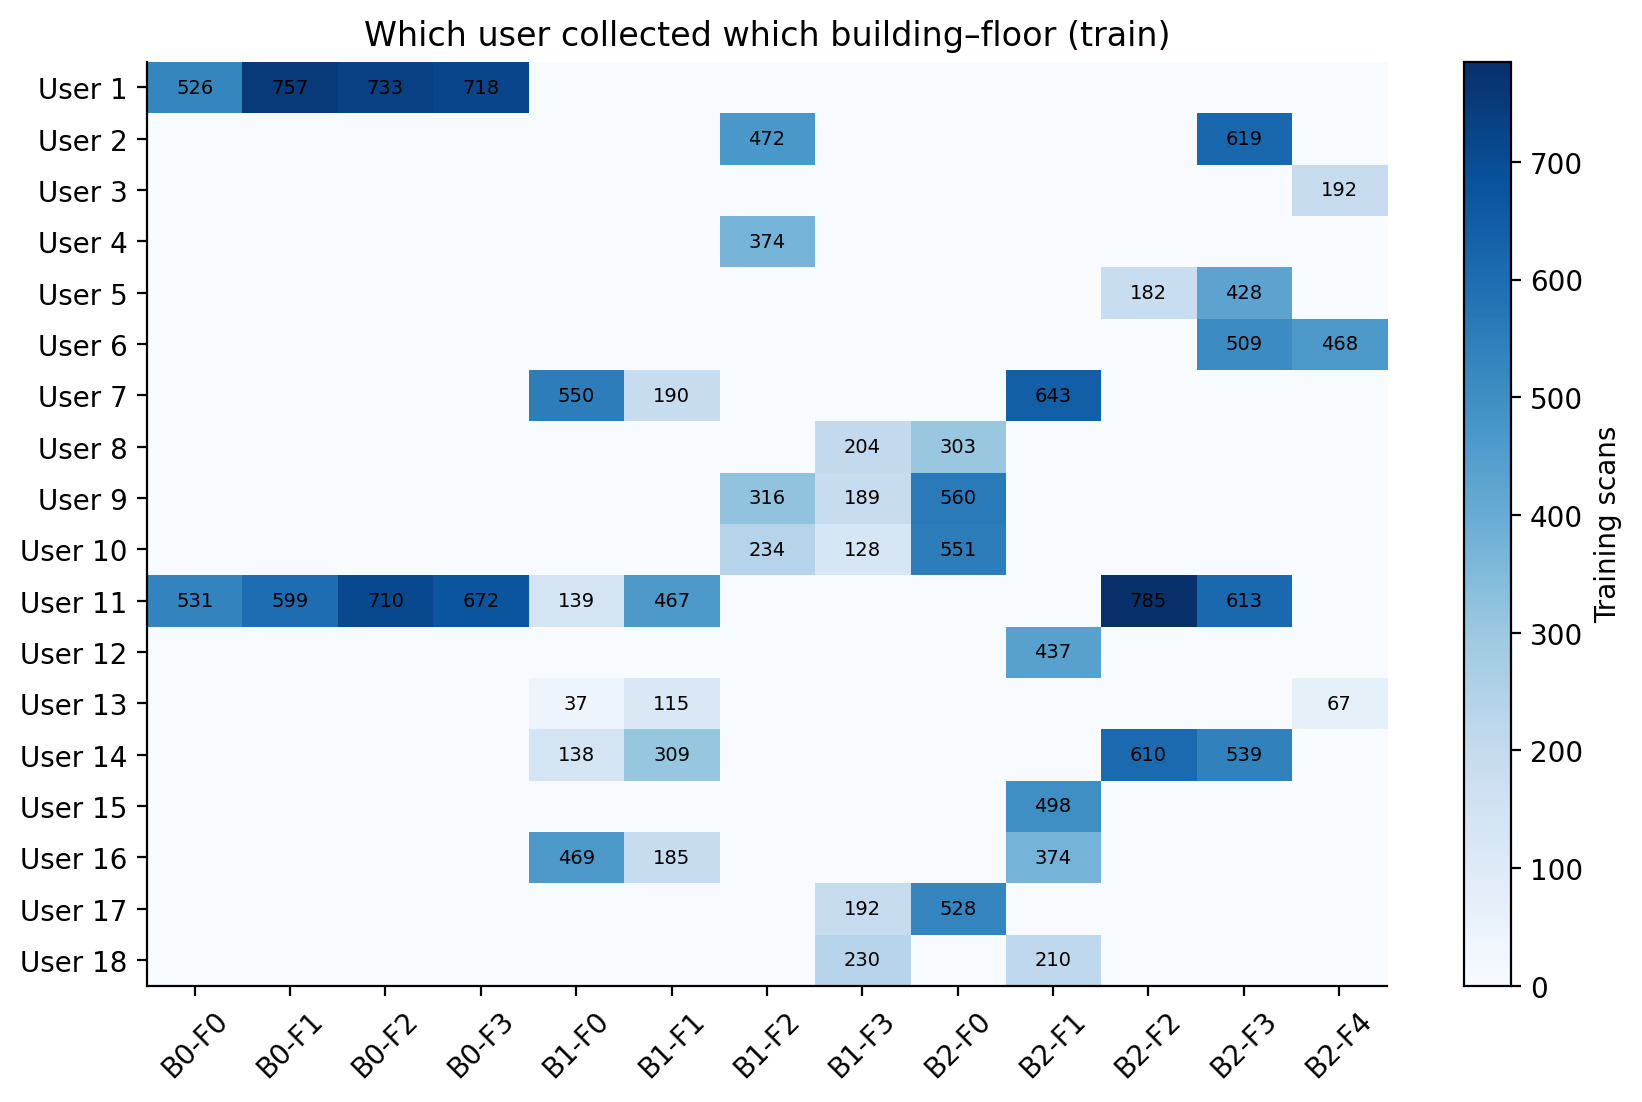
\includegraphics[width=\columnwidth]{eda_user_coverage.png}
\caption{Number of training scans collected by each user in each building--floor combination.}
\label{fig:users}
\end{figure}

% Figures are read from ../results/figures/ (see \graphicspath in main.tex)
% ---------------------------------------------------------------

\subsection{Dataset}

We use the UJIIndoorLoc dataset~\cite{torres2014ujiindoorloc, uci_ujiindoorloc}, a public benchmark for
Wi-Fi fingerprinting collected in three buildings of Universitat Jaume I, Spain. Each row is one Wi-Fi
scan taken by a smartphone. It contains the received signal strength (RSSI) of 520 wireless access
points (WAPs), the true location of the phone, and information about who took the scan, with which
phone, and when.

RSSI values are given in dBm and range from $-104$ (very weak) to $0$ (very strong). An access point
that was not detected is recorded as $+100$. This value is a placeholder, not a measurement, and it
must be handled explicitly because otherwise it would look like the strongest possible signal.

The prediction targets are the building (3 classes) and floor (5 classes), treated as classification,
and the longitude and latitude, treated as regression. The coordinates are projected positions in
metres, so positioning error can be reported in metres. The remaining columns (\texttt{SPACEID},
\texttt{RELATIVEPOSITION}, \texttt{USERID}, \texttt{PHONEID}, \texttt{TIMESTAMP}) are not used as model
inputs; we use them only for quality checks and to design fair validation splits.

The dataset is provided as two files: a training file and a validation file. The labels of the original
competition test set were never released, so, following common practice, we use the validation file
as our held-out test set and do not use it for any modelling decision. Table~\ref{tab:summary}
summarises both files.

\begin{table}[!t]
\centering
\caption{Summary of the two data files}
\label{tab:summary}
\begin{tabular}{lrr}
\toprule
 & \textbf{Train} & \textbf{Validation} \\
\midrule
Scans (rows) & 19{,}937 & 1{,}111 \\
Buildings / floors & 3 / 5 & 3 / 5 \\
Building--floor combinations & 13 & 13 \\
Users / phones & 18 / 16 & -- / 11 \\
Collection period & May--Jun 2013 & Sep--Oct 2013 \\
Signal values $=100$ (not detected) & 96.5\% & 96.8\% \\
Median APs detected per scan & 17 & 15 \\
Scans with no AP detected & 76 & 0 \\
Exact duplicate rows & 637 & 0 \\
Scans after removing duplicates & 19{,}300 & 1{,}111 \\
\bottomrule
\end{tabular}
\end{table}

\begin{figure}[!t]
\centering
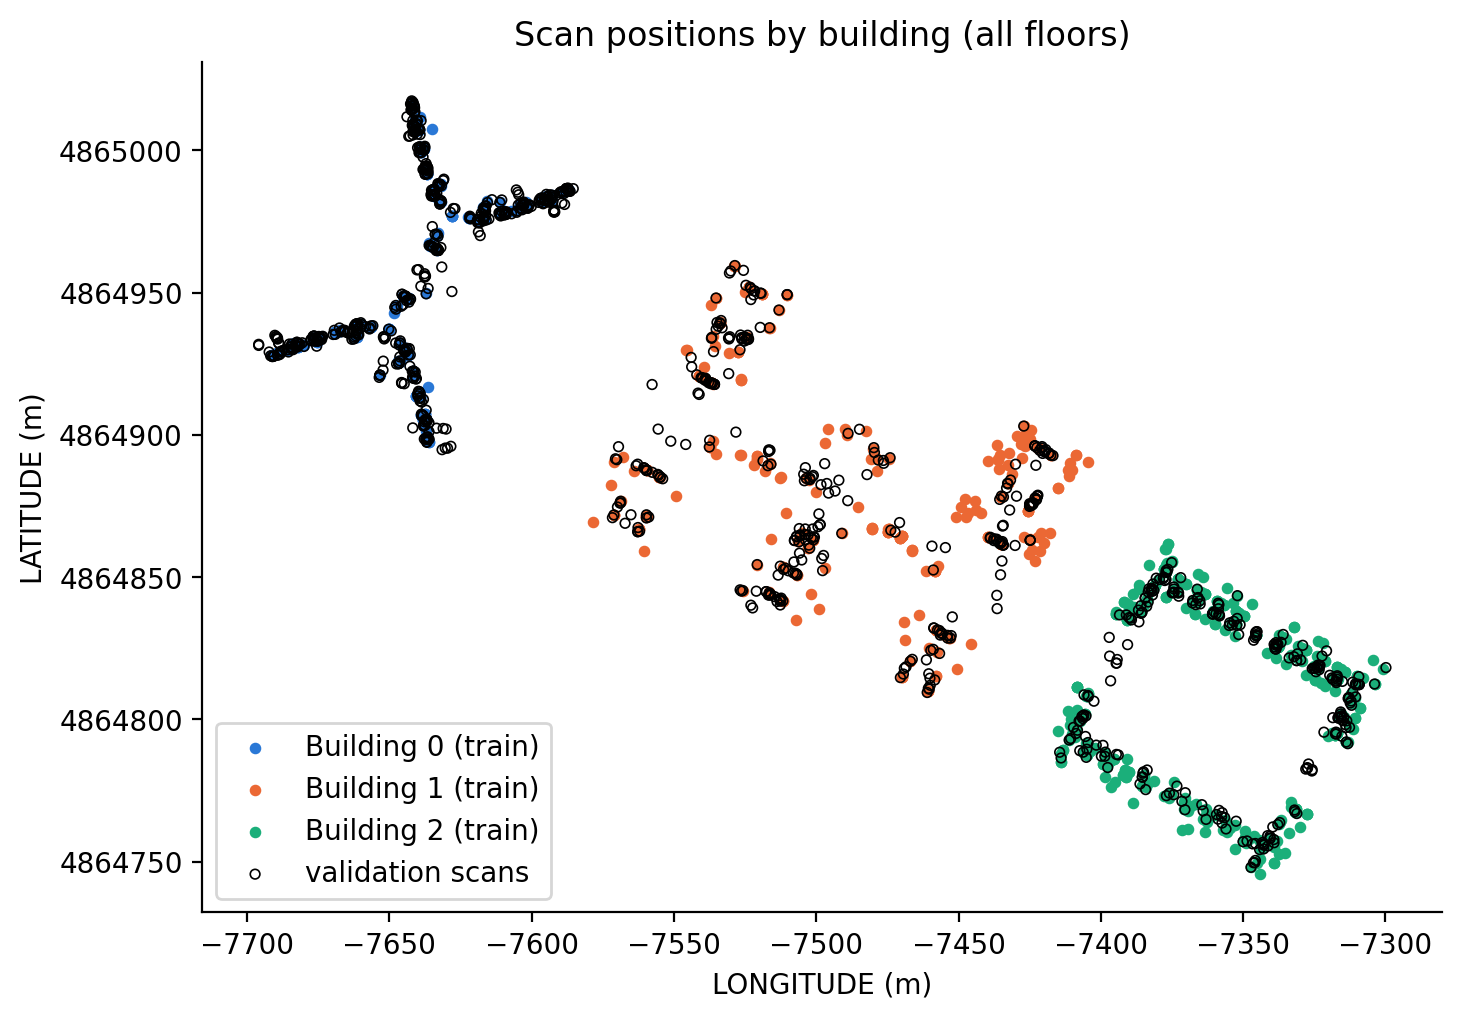
\includegraphics[width=\columnwidth]{eda_map_by_building.png}
\caption{Scan positions in the training file, coloured by building, with validation scans shown as
black circles. The three buildings occupy separate areas of the campus.}
\label{fig:map}
\end{figure}

\subsection{Data Quality}

Table~\ref{tab:quality} lists the quality checks and their outcome. The data is reliable overall: all
real RSSI values lie in the documented range, the labels are valid (floor~4 exists only in
building~2, the only five-floor building), and the three buildings are spatially separate
(Fig.~\ref{fig:map}).

A few issues require preprocessing decisions. First, the training file contains 637 exact duplicate
rows (3.2\%), 622 of them from a single user. None has conflicting labels, but copies falling on both
sides of a split would inflate validation scores, so we remove them. All results below use the remaining
19{,}300 training scans. Second, 73 of these scans detected no access point at all and therefore carry
no information; 59 of them come from a single user and phone, which points to a faulty recording
session. Third, 55 access points are never detected in the training file, so their columns are
constant and can be removed. The same 55 access points do appear in the validation file, while 153
access points seen in training never appear in validation, which shows that the Wi-Fi infrastructure
changed between the two collections.

Finally, 775 readings stronger than $-30$~dBm occur in 492 training scans, whereas the strongest
validation reading is $-34$~dBm. 87\% of these scans come from one device (phone~19), so we treat them
as a device artefact; capping readings at $-30$~dBm removes them.

\begin{table}[!t]
\centering
\caption{Data-quality checks on the training file}
\label{tab:quality}
\setlength{\tabcolsep}{3pt}
\begin{tabular}{p{0.27\columnwidth}p{0.40\columnwidth}p{0.27\columnwidth}}
\toprule
\textbf{Check} & \textbf{Result} & \textbf{Action} \\
\midrule
RSSI range & All real values in $[-104, 0]$ & None \\
Labels & Valid; floor 4 only in building 2 & None \\
Empty scans & 73 (59 from one device) & Remove \\
Duplicates & 637 exact duplicates (622 from one user) & Removed \\
Never-detected APs & 55 constant columns & Drop \\
Very strong readings & 492 scans, 87\% from phone 19 & Cap at $-30$ dBm \\
Validation metadata & User, room and position columns are always 0 & Never use as inputs \\
\bottomrule
\end{tabular}
\end{table}

\subsection{Label Distributions}

Fig.~\ref{fig:buildings} shows that the two files emphasise different buildings: building~2 makes up
47.2\% of the training scans, while building~0 makes up 48.2\% of the validation scans. Overall
validation accuracy is therefore driven mostly by building~0, and we report results per building as
well as overall.

Class imbalance is moderate (Fig.~\ref{fig:classes}). Every building--floor combination has at least
727 training scans, recorded at 50--113 distinct positions with about 20 scans per position. The
largest combination (building~2, floor~3) has 3.7 times as many scans as the smallest (building~2,
floor~4). A classifier that always predicts the most frequent class would reach 47.2\% building
accuracy and 26.1\% floor accuracy; these are the baselines any model must clearly exceed. Because of
the imbalance, we report macro-F1 alongside accuracy.

\begin{figure}[!t]
\centering
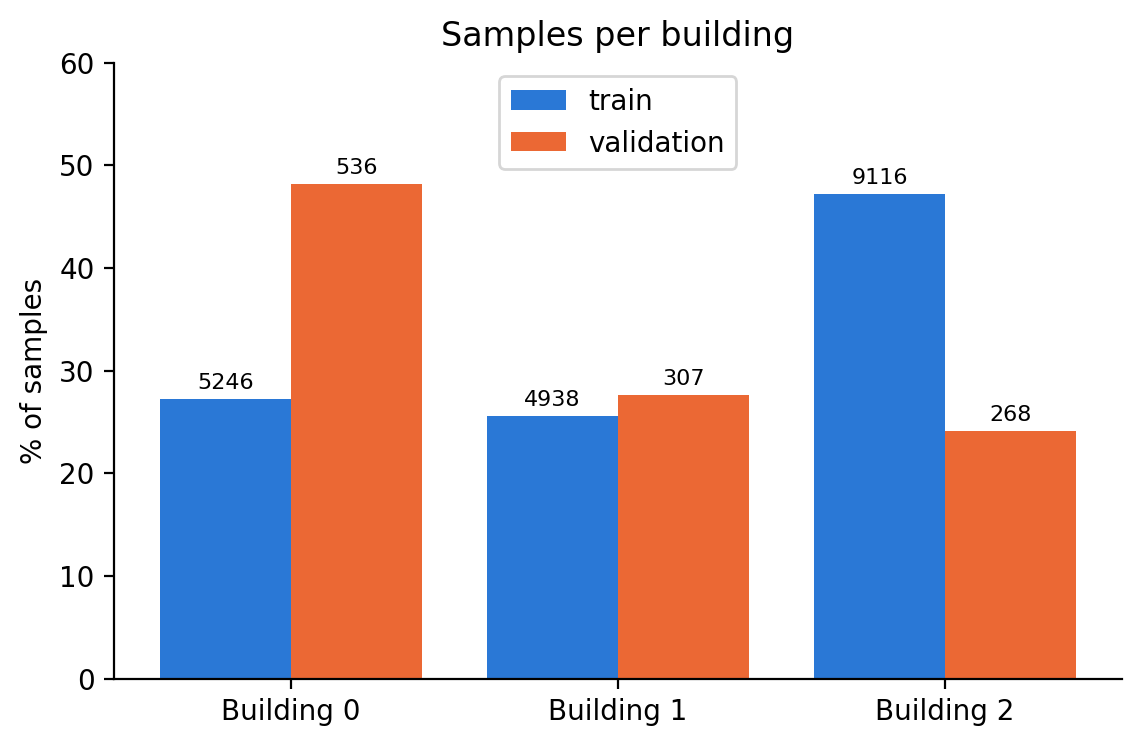
\includegraphics[width=0.9\columnwidth]{eda_samples_per_building.png}
\caption{Share of scans per building in each file (counts above the bars).}
\label{fig:buildings}
\end{figure}

\begin{figure}[!t]
\centering
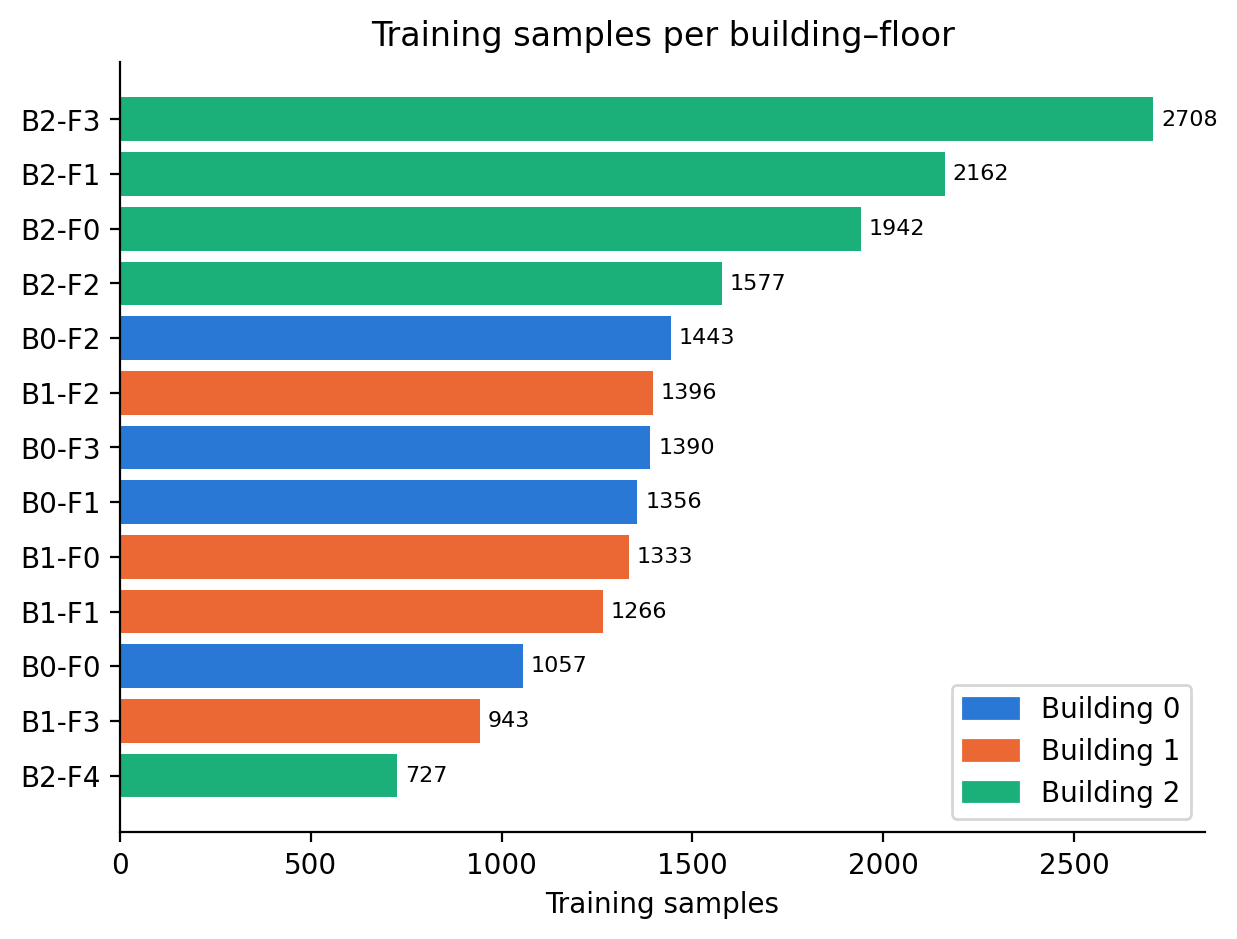
\includegraphics[width=0.9\columnwidth]{eda_building_floor_classes.png}
\caption{Training scans for each of the 13 building--floor combinations.}
\label{fig:classes}
\end{figure}

\subsection{Signal Characteristics}

The data is extremely sparse: 96.5\% of all signal values are ``not detected'', and a typical scan
picks up only 17 of the 520 access points. Among the real readings, most signals are weak, with a median
of $-82$~dBm in training and $-80$~dBm in validation (Fig.~\ref{fig:rssi}). Since the weakest real
reading is $-104$~dBm, the placeholder $+100$ should be replaced by a lower value such as $-110$~dBm,
which keeps the natural order ``not detected'' $<$ ``weakest detected''.

The number of detected access points also carries location information: scans in building~2 detect a
median of 19 access points, compared with 15--16 in buildings~0 and~1. This motivates aggregate
features for our models (number of detected access points and strongest signal per scan).

\begin{figure}[!t]
\centering
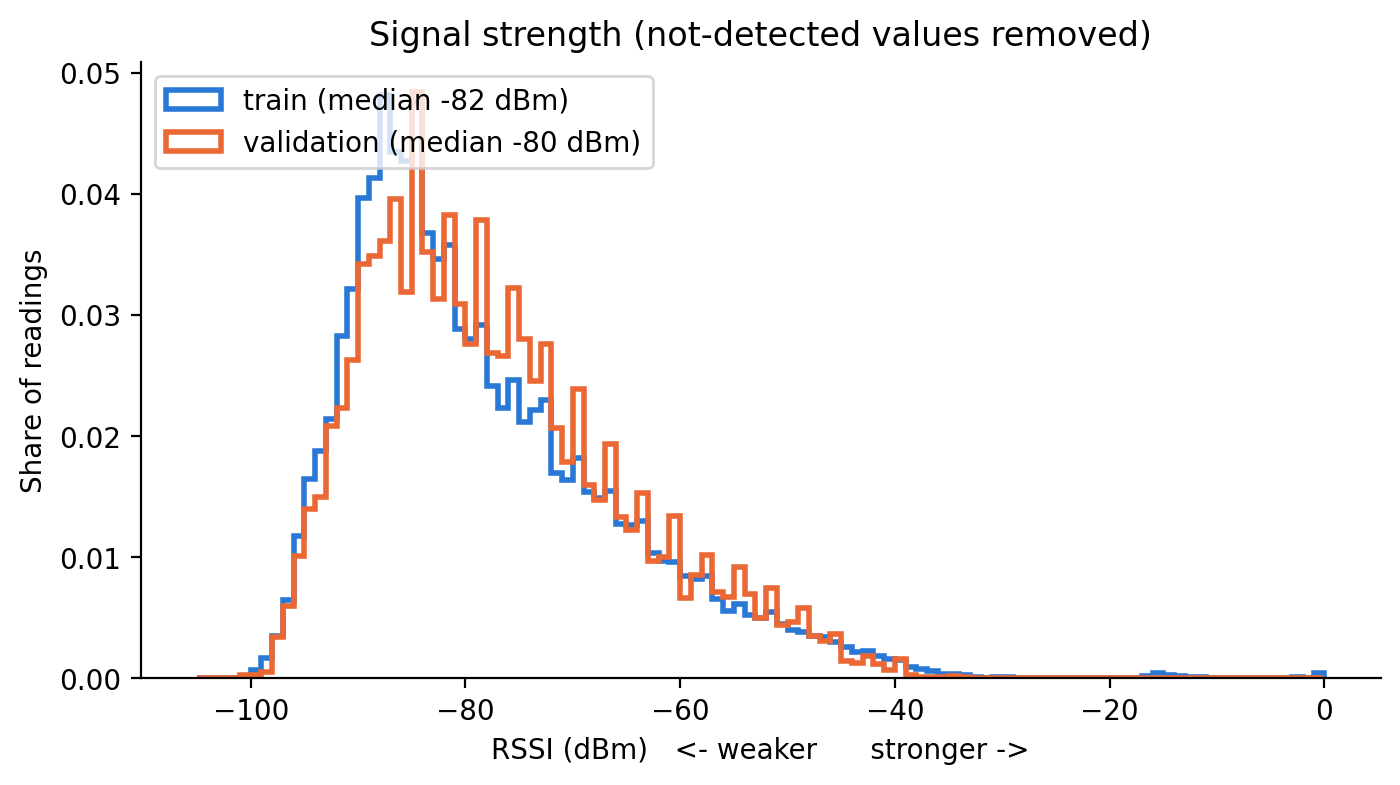
\includegraphics[width=\columnwidth]{eda_rssi_distribution.png}
\caption{Distribution of real RSSI readings (placeholder values removed).}
\label{fig:rssi}
\end{figure}

\subsection{Differences Between the Training and Validation Files}

The two files differ in several ways, so lower scores on the validation file than within the training
file are expected:
\begin{itemize}
\item \textbf{Time:} the files were collected 91 days apart, and each is dominated by a single session
(72.8\% of training scans on one day, 63\% of validation scans on another).
\item \textbf{Phones:} only 2 of the 11 phones in the validation file were used in training. Phones
differ by about 15~dB in typical reported signal strength and detect a median of 9 to 32 access points
per scan (Fig.~\ref{fig:phones}).
\item \textbf{Access points:} the detection rates of individual access points are only moderately
correlated between the files ($r = 0.65$), and 55 access points appear only in validation.
\item \textbf{Signal distributions:} a Kolmogorov--Smirnov test shows a moderate shift in the number of
access points per scan (KS $= 0.12$) and only small shifts in signal strength (KS $= 0.07$--$0.08$).
\end{itemize}

Despite these differences, the validation scans are well covered spatially: the median distance from a
validation scan to the nearest training position on the same floor is 0.9~m, and 90\% are within 4.6~m.
However, 35 validation scans (3.2\%) are more than 10~m from any training position, and we expect the
largest positioning errors there.

\begin{figure*}[!t]
\centering
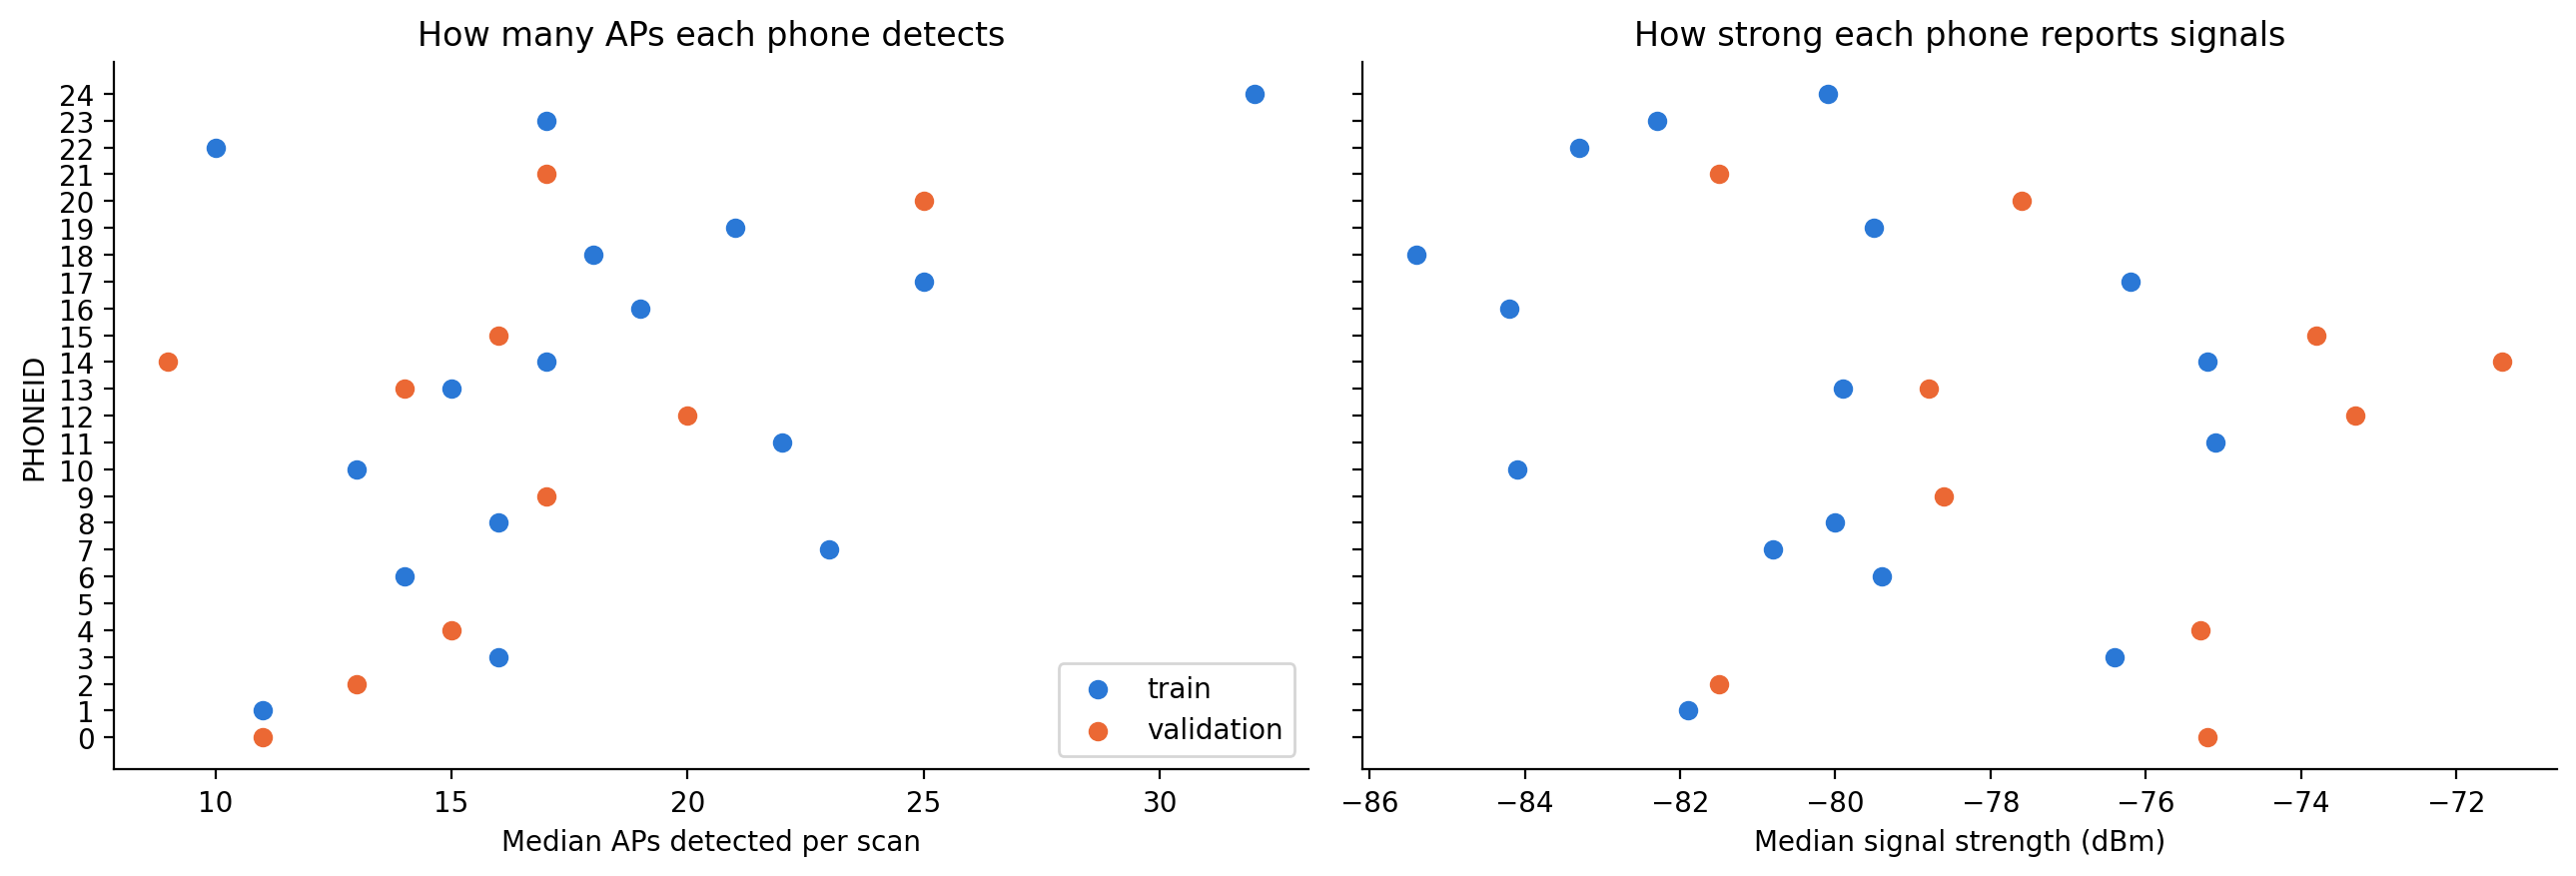
\includegraphics[width=0.85\textwidth]{eda_phone_differences.png}
\caption{Differences between phones (phones with at least 20 scans). Left: median number of access
points detected per scan. Right: median signal strength. Most validation phones (orange) were never
used in training.}
\label{fig:phones}
\end{figure*}

\subsection{Leakage Risks and Validation Strategy}

Each training position was scanned about 20 times, and each user collected only 1 to 8 of the 13
building--floor combinations using exactly one phone (Fig.~\ref{fig:users}). These properties determine
how models can be validated fairly. Table~\ref{tab:leakage} shows, for different 5-fold splits of the
training file, the share of test-fold scans whose exact position also appears in the training fold.

\begin{table}[!t]
\centering
\caption{Share of test-fold scans at a position already seen in training (5-fold splits of the training file)}
\label{tab:leakage}
\begin{tabular}{lr}
\toprule
\textbf{Split} & \textbf{Positions already seen} \\
\midrule
Random 5-fold & 100.0\% \\
Grouped by user & 78.2\% \\
Grouped by position & 0.0\% \\
\bottomrule
\end{tabular}
\end{table}

A random split places every test scan at a position the model has already seen, which would give
unrealistically optimistic scores. We therefore adopt the following protocol:
\begin{enumerate}
\item \textbf{Final results:} train on the training file and evaluate once on the validation file. No
validation scan is identical to a training scan, so this split has no direct leakage.
\item \textbf{Hyperparameter tuning:} 5-fold cross-validation within the training file, grouped by
position.
\item \textbf{Robustness:} 5-fold cross-validation grouped by user. Since each user used one phone, this
also tests generalisation to an unseen device.
\end{enumerate}
In addition, all preprocessing steps (placeholder replacement, scaling and column removal) are fitted on
the training file only, and the room-level columns \texttt{SPACEID} and \texttt{RELATIVEPOSITION} are
never used as inputs because they directly encode the location.

\begin{figure}[!t]
\centering
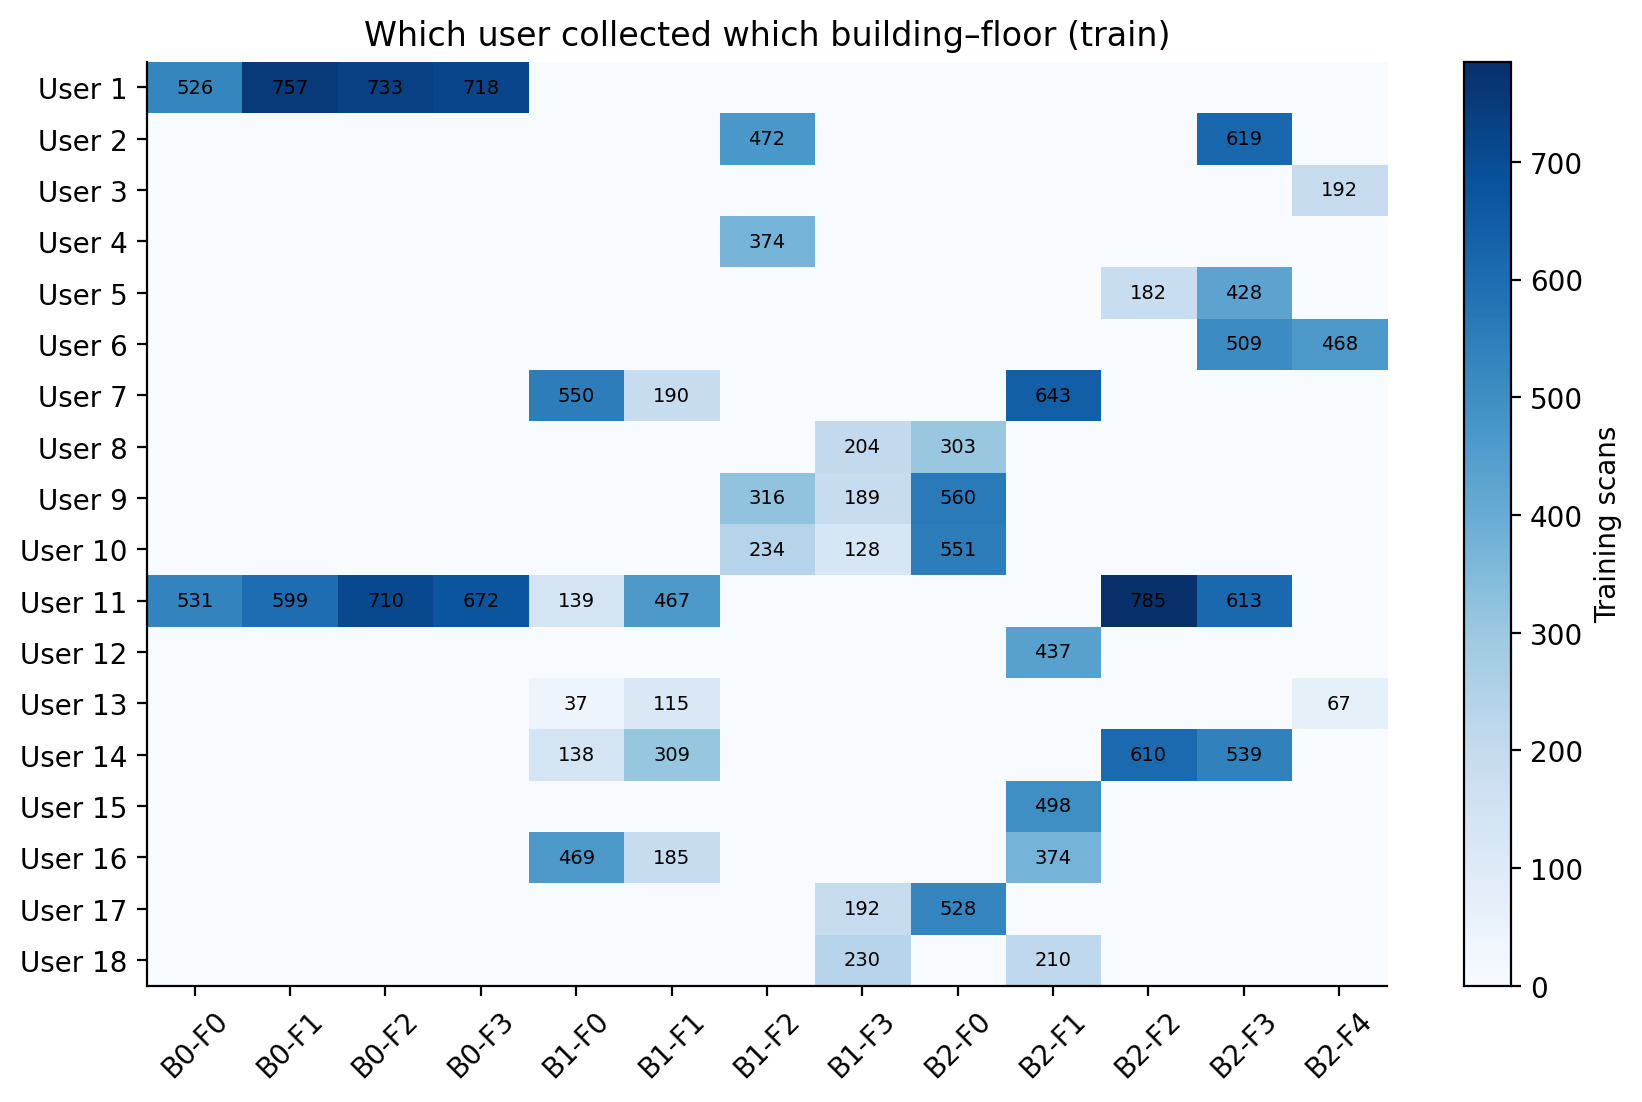
\includegraphics[width=\columnwidth]{eda_user_coverage.png}
\caption{Number of training scans collected by each user in each building--floor combination.}
\label{fig:users}
\end{figure}
